% ============================================================================ %
%
%           Šablona bakalářské/diplomové práce
%
% Autor:    Ing. Jozef Říha (2006-05-04), od té doby šablonu udržuje
%           Ing. Pavel Tomášek, Ph.D. (tomasek@utb.cz)
%
% Verze:    2021-05-04
%
% Kódování: UTF-8 (kontrolní řetězec: žluťoučký kůň úpěl ďábelšké ódy)
%
% Sazba:    pdflatex prace.tex && pdflatex prace.tex
%           (nutné dvakrát pro korektní vložení citací a jiných referencí),
%           v případě umístění literatury do externího bib souboru je třeba volat
%           pdflatex prace.tex && bibtex prace && pdflatex prace.tex && pdflatex prace.tex
%
% Tip:      Ve správně vysázeném českém textu by na konci řádku neměla zůstant
%           samotná jednopísmenná předložka či spojka. Na takové místo se vkládá
%           nezalomitelná mezera pomocí symbolu ~. Existuje program, který umí
%           zpracovat celý TeX dokument najednou podle českých konvencí:
%           http://petr.olsak.net/ftp/olsak/vlna/
%
% Pozor:    Vzhledem k požadovanému standardu PDF/A nesmí vložené obrázky 
%           obsahovat alfa kanál (průhlednost).
%
% ============================================================================ %


\documentclass[a4paper,12pt]{article}

% Definice vzhledu a nastavení se načítá z následujícího souboru (netřeba editovat)
% ============================================================================ %
% Tento dokument není zpravidla třeba editovat,
% obsahuje nastavení balíčků, vzhledu, stylů.
%
% Kódování: UTF-8 (žluťoučký kůň úpěl ďábelšké ódy)
% ============================================================================ %


% ============================================================================ %
% BALÍČKY

%\usepackage[czech,english]{babel} % volba při kompilaci latexem (vyžaduje texlive-lang), zakomentovano, nastavovanu prikazem \nastavjazyk
\usepackage[T1]{fontenc}% definice vnitřního kódování
\usepackage[utf8]{inputenc} % slouží pro definici kódování (při problémech zkusit zaměnit utf8x za utf8)
\usepackage{color}		% umožňuje použití barev
\usepackage{graphicx}	% rozšíření práce s grafikou
\usepackage{amsmath}	% balíček pro pokročilejší matematiku
\usepackage{fancyhdr}	% detailnější nastavení záhlaví a zápatí
\usepackage{tocloft}	% umožňuje pohodlné nastavení vzhledu obsahu, seznamu tabulek či obrázků
\usepackage{textcase}	% změna VeLiKoStI PíSmA
\usepackage{ifthen} 	% balíček umožňující skladby if, then -- využijeme při definici nadpisů
\usepackage{setspace}	% balíček umožňující nastavit řádkování na 1, 1.5, 2
\usepackage{ccaption}	% vylepšení práce s popisky obrázků či tabulek
\usepackage{sectsty}	% pro nastavení vzhledu nadpisů
\usepackage[srcstyle=leftnumhang,linenumbersep={\ }]{examplep} % pokročilejší sazba programového kódu
\usepackage{url}		% balíček pro vysázení internetové adresy stylem verbatim s vylepšeným řádkovým zlomem
\usepackage{afterpage}
%\usepackage{layout}	% zobrazí nastavení tiskového zrcadla (příkaz \layout)
%\usepackage{times}		% balíček pro použití fontu times
%\usepackage{verbatim}	% vysází text bez formátování, tak jak je zapsán v souboru
%\usepackage{indentfirst} % definuje odsazení prvního řádku odstavce
%\usepackage{makeidx}	% vytvoří rejstřík
\usepackage[pdftex,pdfa,hidelinks,breaklinks]{hyperref}	% vytváří křížové odkazy
%\usepackage{multicol}	% vícesloupcová sazba
%\usepackage{flafter}	% zajistí, aby se plovoucí objekty objevovali až za jejich umístěním v textu
\usepackage{chngcntr}	% Umožňuje změnu nastavení číslování obrázků, tabulek i rovnic
\usepackage{etoolbox}	% Tool-box for LaTeX programmers
\usepackage[labelsep=space,tableposition=bottom,justification=centering]{caption} % Přenastavení popisků u figur a tabulek
\usepackage{xmpincl}	% Pro aplikaci standardu PDF/A
\usepackage{hyperxmp}	% Pro aplikaci standardu PDF/A

%\pdfminorversion=4
%\pdfobjcompresslevel=0


% ---------------------------------------------------------------------------- %

% NASTAVENÍ TISKOVÉHO ZRCADLA

\newcommand{\valueTextHeight}{242mm}	% výška tiskového zrcadla
\newcommand{\valueTextWidth}{155mm}	% šířka tiskového zrcadla
\newcommand{\valueVOffset}{-1.61cm}	% vertikální posunutí tiskového zrcadla
\newcommand{\valueSideMargin}{0.96cm}	% levý okraj
\newcommand{\valueHeadHeight}{0.6cm}	% záhlaví
\newcommand{\valueHeadSep}{1cm}	% záhlaví

\textheight=\valueTextHeight
\textwidth=\valueTextWidth
\voffset=\valueVOffset
%\voffset=-1in
%\topmargin=-2.9cm

\oddsidemargin=\valueSideMargin
\evensidemargin=\valueSideMargin

\headheight=\valueHeadHeight
\headsep=\valueHeadSep

% nastavení zápatí
\footskip=1ex
\cfoot{}
% "vypnout" poznámky na okrajích
\marginparpush=0mm
\marginparwidth=0mm
\marginparsep=0mm

\pagestyle{fancy}

% Nastavení obalujících okrajů okolo popisků figur a tabulek
\captionsetup[figure]{aboveskip=5pt}
\captionsetup[figure]{belowskip=0pt}
\captionsetup[table]{aboveskip=0pt}
\captionsetup[table]{belowskip=5pt}


% ============================================================================ %
% NASTAVENÍ PÍSMA, ODSTAVCE, ROVNIC, POZNÁMEK

\parindent=0em				% velikost odstavcové zarážky na nulu
\def\thefootnote{\arabic{footnote})}	% poznámka pod čarou se závorkou
\onehalfspacing % nastavím řádkování tímto způsobem nebo \renewcommand{\baselinestretch}{1.5} ??
\setlength{\parskip}{3pt}		% vertikální mezera mezi nadpisy
%\def\label#1{{\sf ! #1 ! }}		% možnost zobrazení všech \label{}


% ============================================================================ %
% NASTAVENÍ ČÍTAČŮ

\setcounter{tocdepth}{3} % do obsahu se ukládají pouze první dvě úrovně kapitol


% ============================================================================ %
% PDF/A STANDARD

% http://www.mathstat.dal.ca/~selinger/pdfa/
% https://blog.zhaw.ch/icclab/creating-pdfa-documents-for-long-term-archiving/
% http://support.river-valley.com/wiki/index.php?title=Generating_PDF/A_compliant_PDFs_from_pdftex

% Prerequisites: pdflatex, hyperref, xmpincl
% pdfTeX at least in version 1.40.15 (in Linux add repository ppa:jonathonf/texlive, update and upgrade texlive-full)
%
% Validator: http://pdfa.k.utb.cz:8080/ https://www.pdf-online.com/osa/validate.aspx

% \convertDate converts D:20080419103507+02'00' to 2008-04-19T10:35:07+02:00
\def\convertDate{%
	\getYear
}
{\catcode`\D=12
 \gdef\getYear D:#1#2#3#4{\edef\xYear{#1#2#3#4}\getMonth}
}
\def\getMonth#1#2{\edef\xMonth{#1#2}\getDay}
\def\getDay#1#2{\edef\xDay{#1#2}\getHour}
\def\getHour#1#2{\edef\xHour{#1#2}\getMin}
\def\getMin#1#2{\edef\xMin{#1#2}\getSec}
\def\getSec#1#2{\edef\xSec{#1#2}\getTZh}
\def\getTZh +#1#2{\edef\xTZh{#1#2}\getTZm}
\def\getTZm '#1#2'{%
	\edef\xTZm{#1#2}%
	\edef\convDate{\xYear-\xMonth-\xDay T\xHour:\xMin:\xSec+\xTZh:\xTZm}%
}
\expandafter\convertDate\pdfcreationdate

\pdfminorversion 4

\immediate\pdfobj stream attr{/N 3} file{graphics/sRGBIEC1966-2.1.icm}
\pdfcatalog{%
	/OutputIntents [ <<
	/Type /OutputIntent
	/S/GTS_PDFA1
	/DestOutputProfile \the\pdflastobj\space 0 R
	/OutputConditionIdentifier (sRGB IEC61966-2.1)
	/Info(sRGB IEC61966-2.1)
 >> ]
}

\providecommand{\xmpOrg}{Tomas Bata University in Zlín, Czech Republic}
\providecommand{\xmpProducer}{}
\providecommand{\xmpDoi}{}
\providecommand{\xmpJournalnumber}{}
\providecommand{\xmpVolume}{}
\providecommand{\xmpIssue}{}
\providecommand{\xmpCoverDisplayDate}{}
\providecommand{\xmpCoverDate}{}
\providecommand{\xmpJournaltitle}{}
\providecommand{\xmpFirstpage}{}
\providecommand{\xmpLastpage}{}
\providecommand{\xmpAuthoritativeDomain}{}
\providecommand{\xmpCreatorTool}{}%pdfTeX

\newcommand{\aplikujpdfa}{
	\ifczech
		\providecommand{\xmpTitle}{\nazevcz}
		\providecommand{\xmpAuthor}{\autor}
		\providecommand{\xmpKeywords}{\klicovaslovacz}
		\hypersetup{
			pdftitle={\nazevcz},
			pdfauthor={\autor},
			pdfsubject={\abstraktcz},
			pdfkeywords={\klicovaslovacz},
			%pdfproducer={pdfTeX-1.40.20},
			pdflang=la,
			pdfapart=3,
			pdfaconformance=B,
			pdflang={cz}
		}
	\else \ifenglish
		\providecommand{\xmpTitle}{\nazeven}
		\providecommand{\xmpAuthor}{\autor}
		\providecommand{\xmpKeywords}{\klicovaslovaen}
		\hypersetup{
			pdftitle={\nazeven},
			pdfauthor={\autor},
			pdfsubject={\abstrakten},
			pdfkeywords={\klicovaslovaen},
			%pdfproducer={pdfTeX-1.40.20},
			pdflang=la,
			pdfapart=3,
			pdfaconformance=B,
			pdflang={en}
		}
	\fi \fi
	
	\makeatletter
	\includexmp{tex/pdfa-1b}
	\makeatother
}


% ============================================================================ %
% UŽIVATELSKÉ STYLY

% Styl nn = nečíslovaný nadpis (je vysázený v obsahu)
\def\nn#1{\clearpage\phantomsection\addcontentsline{toc}{section}{#1}\section*{\MakeTextUppercase{#1}}}

% Styl nm = nečíslovaný nadpis (není vysázený v obsahu)
\def\nm#1{\clearpage\section*{\MakeTextUppercase{#1}}}

% Styl ns = nečíslovaný nadpis na stejné stránce (není vysázený v obsahu)
\def\nns#1{\section*{\MakeTextUppercase{#1}}}

% Styl n{ur}{nadp} pro nadpisy, kde ur je číslo úrovně a nadp je text nadpisu
\def\n#1#2{
	
	\ifthenelse{#1=1}{
		\sectionfont{\normalsize\MakeUppercase}
		\clearpage\section{#2}
		\sectionfont{\normalsize}
		}{
		\ifthenelse{#1=2}{\subsection{#2}}{
			\ifthenelse{#1=3}{\subsubsection{#2}}{\paragraph{\itshape\bfseries{#2}}
}}}}

% Styl pro obrázky
% \obr{popisek}{label}{rozměr (0.0 - 1.0)}{soubor}
\def\obr#1#2#3#4{
	\begin{figure}[h]
		\centering
		\includegraphics[width=#3\linewidth]{#4}
		%\captionwidth{#3\linewidth}
		%\changecaptionwidth
		\captionsetup{width=#3\linewidth}
		\caption{#1}
		\label{#2}
	\end{figure}
}

% Styl pro tabulky
% \tab{popisek}{label}{rozměr (0.0 - 1.0)}{definice sloupců}{obsah} 
\def\tab#1#2#3#4#5{
	\begin{table}[h]
		%\captionwidth{#3\linewidth}
		%\changecaptionwidth
		\captionsetup{width=#3\linewidth}
		\caption{#1}
		\label{#2}
		\centering
		\begin{tabular}{#4}
			#5
		\end{tabular}
	\end{table}
}

% Styl pro tabulky v příloze
% \tabpri{popisek}{definice sloupců}{data tabulky}
\def\tabpri#1#2#3{
	\begin{table}[h]
	\begin{center}
	#1
	\end{center}
	\begin{center}
	\begin{tabular}{#2}
	#3
	\end{tabular}
	\end{center}
	\end{table}
}
	
% Styl pro tabulky z MS Excelu exportované do EPS
% \extab{popisek}{rozměr (0.0 - 1.0)}{soubor}
\def\extab#1#2#3{
	\begin{table}
	%\captionwidth{#2\linewidth}
	%\changecaptionwidth
	\captionsetup{width=#2\linewidth}
	\caption{#1}
	\begin{center}
	\includegraphics[width=#2\linewidth]{#3}
	\end{center}
	\end{table}
}

% Styl pro rovnice
% \rov[klíčové slovo]{rovnice}
\newcommand{\rov}[2][chybejici rovnice]{
	\begin{equation}
	#2
	\label{#1}
	\end{equation}
}
	
% Příkaz pro vysázení seznamu obrázků
\def\seznamobr{
	\clearpage
	\phantomsection
	\ifczech
		\addcontentsline{toc}{section}{Seznam obrázků}
	\else \ifenglish
		\addcontentsline{toc}{section}{List of Figures}
	\fi \fi
	\listoffigures
	\clearpage
}

% Příkaz pro vysázení seznamu tabulek
\def\seznamtab{
	\clearpage
	\phantomsection
	\ifczech
		\addcontentsline{toc}{section}{Seznam tabulek}
	\else \ifenglish
		\addcontentsline{toc}{section}{List of Tables}
	\fi \fi
	\listoftables
	\clearpage
}

\newcommand{\OdsazovaniOdstavcuStart}[0]{
	\ifenglish
		\setlength{\parskip}{5mm} % English indentation of paragraphs
	\else \ifczech
		\setlength{\parindent}{5mm} % Czech indentation of paragraphs
	\fi \fi
}

\newcommand{\OdsazovaniOdstavcuStop}[0]{
	\ifenglish
		\setlength{\parskip}{0mm} % English indentation of paragraphs
	\else \ifczech
		\setlength{\parindent}{0mm} % Czech indentation of paragraphs
	\fi \fi
}

% Příkaz pro vysázení seznamu literatury
\newcommand{\seznamlit}[1]{
	\clearpage
	\phantomsection
	\ifczech
		\addcontentsline{toc}{section}{Seznam použité literatury}
	\else \ifenglish
		\addcontentsline{toc}{section}{References}
	\fi \fi
	\begin{thebibliography}{99}
	#1
	\end{thebibliography}
}

\newcommand{\seznamlitbib}{
	\bibliographystyle{\ifenglish tex/czechiso-en\else\ifczech tex/czechiso-cz\fi\fi} % Respects the norm of ČSN ISO 690
	\newpage
	\clearpage
	%\cleardoublepage
	\phantomsection
	\addcontentsline{toc}{section}{\ifenglish References \else \ifczech Seznam použité literatury \fi \fi}
	\bibliography{tex/literatura}
}

% Příkaz pro přípravu seznamu použitých zkratek a symbolů
\newcommand{\seznamzkr}{
	\ifczech
		\nn{Seznam použitých symbolů a zkratek}
	\else \ifenglish
		\nn{List of Abbreviations}
	\fi \fi
}

% Příkaz \cast jako alternativa k \part
\def\cast#1{
	\clearpage
	\part{#1}
}

% Příkaz \obsah vysází obsah v daném místě
\def\obsah{
	\deaktivujZahlavi
	\clearpage
	\thispagestyle{empty}
	\tableofcontents
	\clearpage
	\pagestyle{fancy}
	\aktivujZahlavi
}

% Zkrácení stylu \textbf na \b
\def\b#1{
	\textbf{#1}
}

% \bi = tučná kurzíva
\newcommand{\bi}[1]{\textbf{\textit{#1}}}

% \it = kurzíva
\renewcommand{\it}[1]{\textit{#1}}

% Nastaveni nezobrazovani zahlavi dokumentu
\newcommand{\deaktivujZahlavi}{
	\lhead{}
	\rhead{}
	\renewcommand{\headrulewidth}{0pt}
}

\newcommand{\zadani}{
	\clearpage
	\thispagestyle{empty}
	\voffset=\valueVOffset\evensidemargin=\valueSideMargin\oddsidemargin=\valueSideMargin\headsep=\valueHeadSep\headheight=\valueHeadHeight\setlength{\parskip}{3pt}\textheight=\valueTextHeight\textwidth=\valueTextWidth
    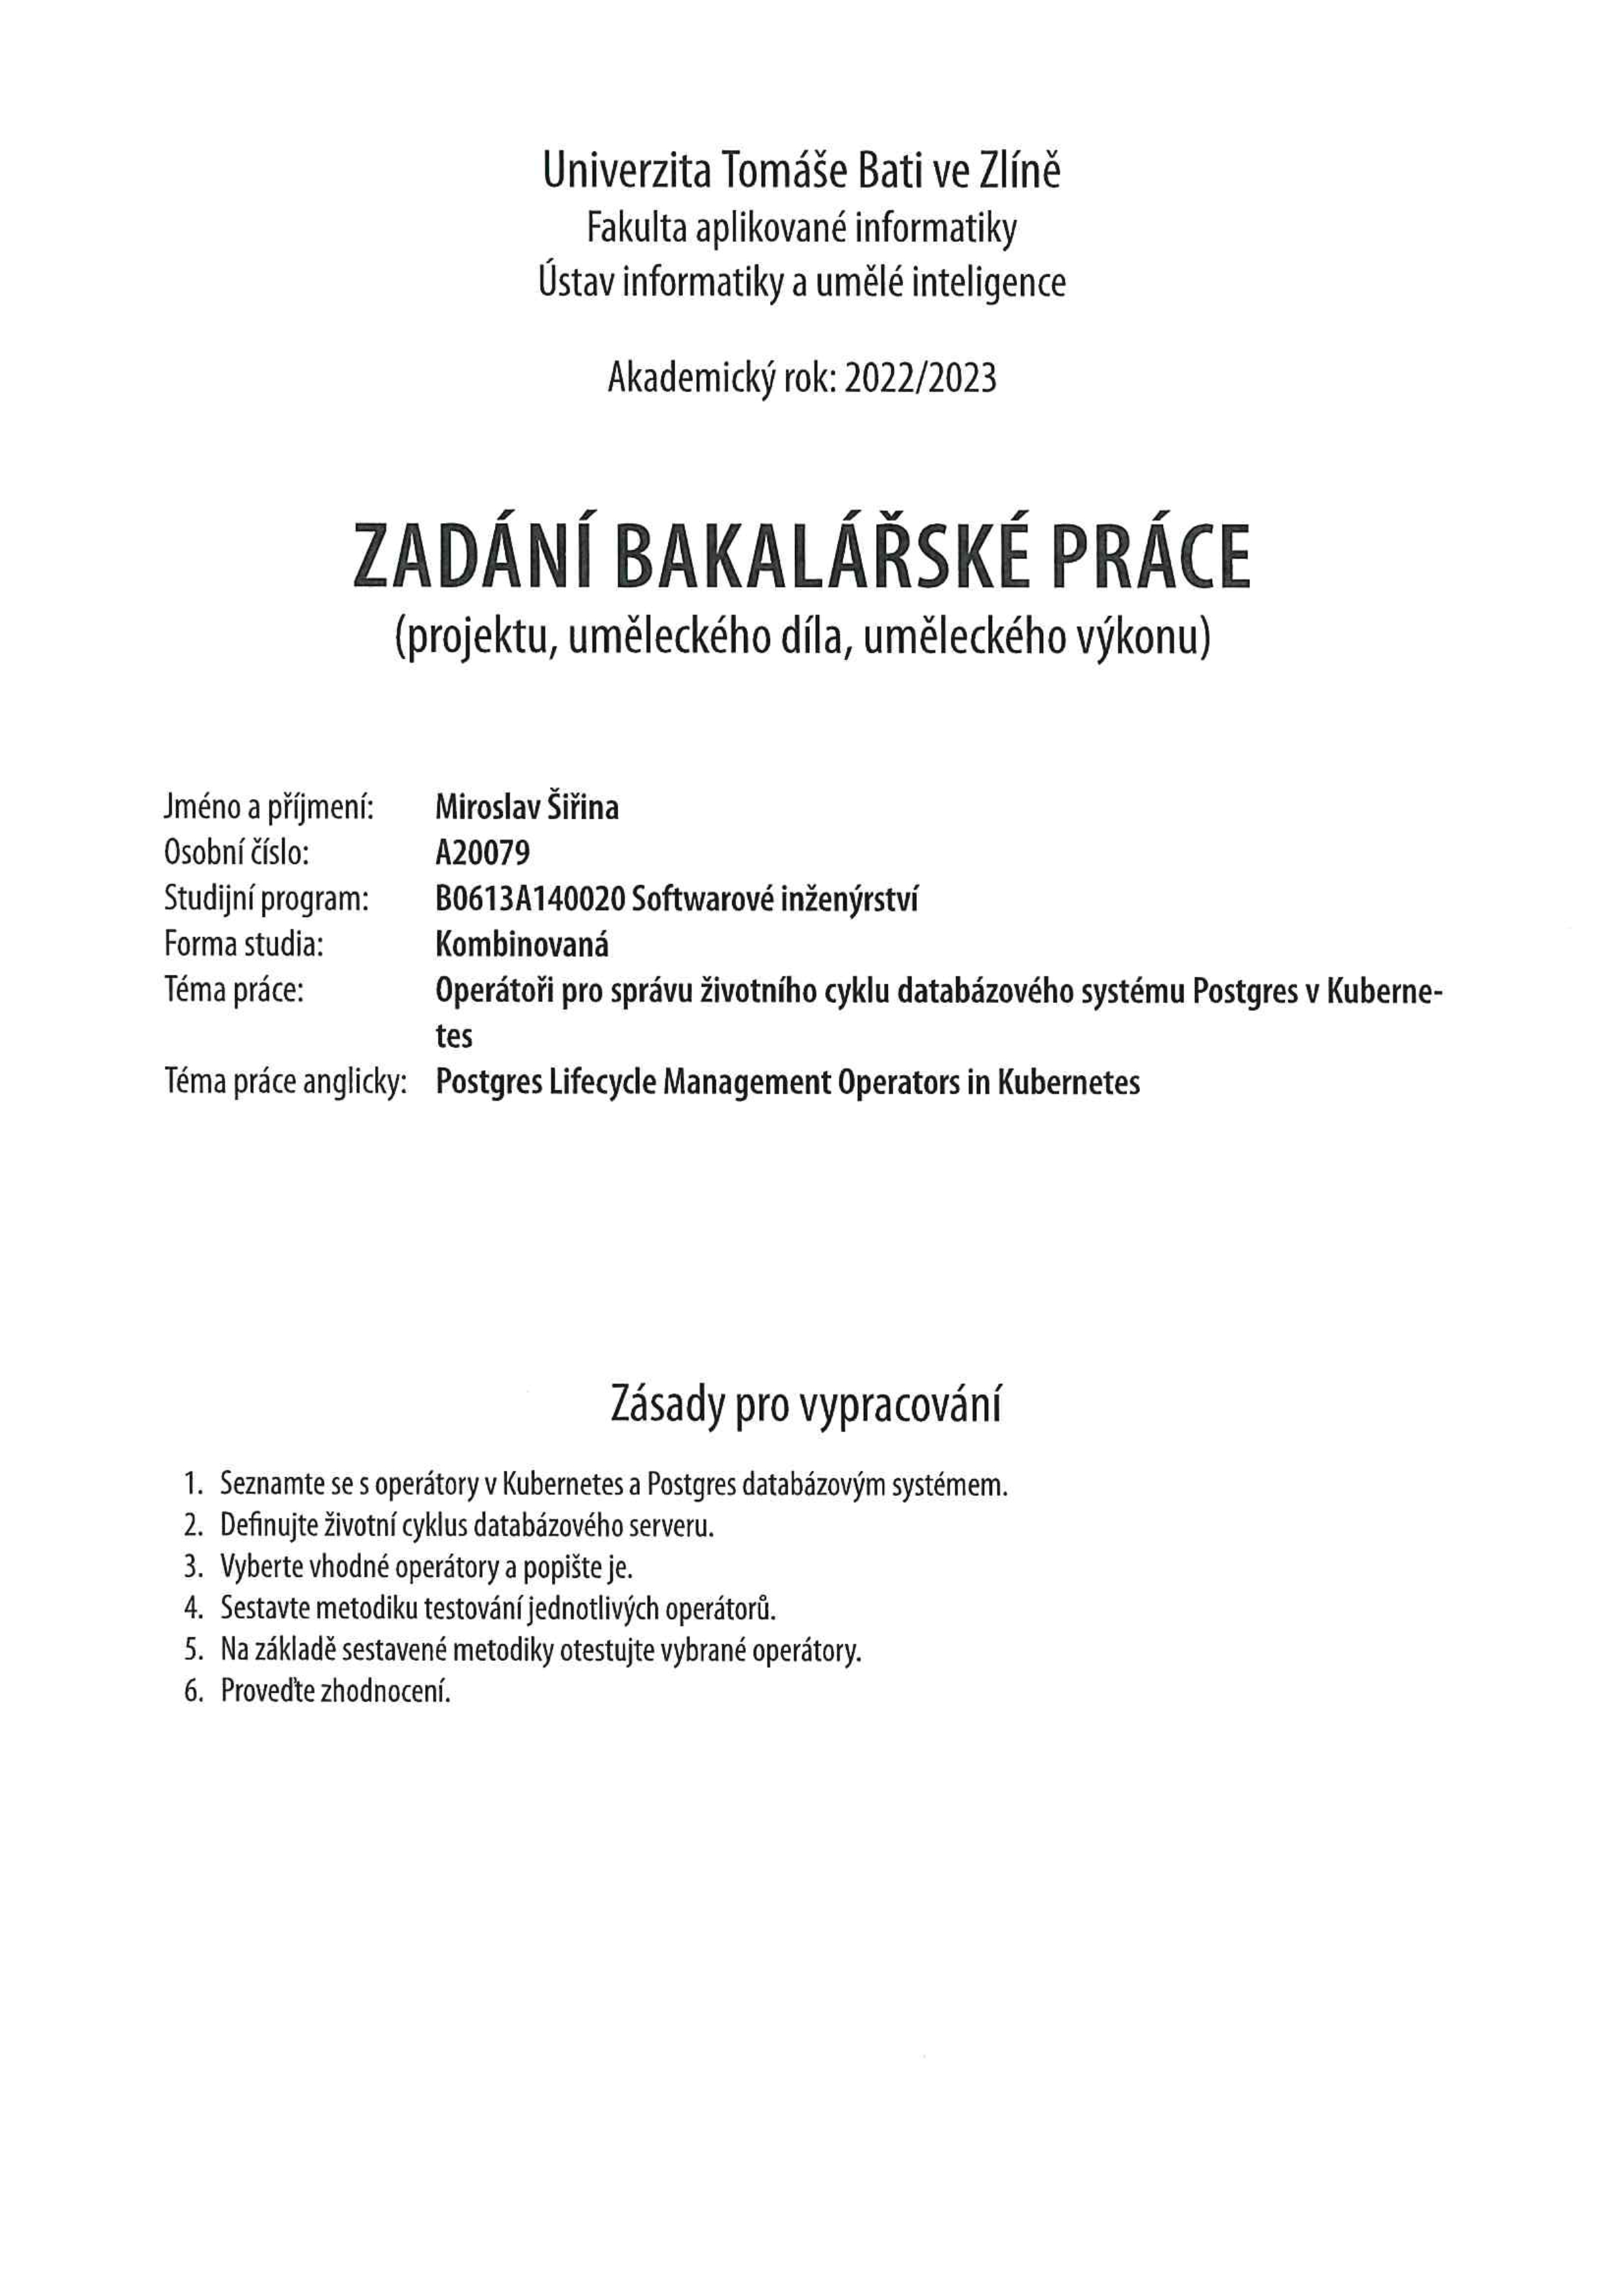
\includegraphics[width=160mm]{graphics/zadani_p1.jpg}

    \clearpage
	\thispagestyle{empty}
	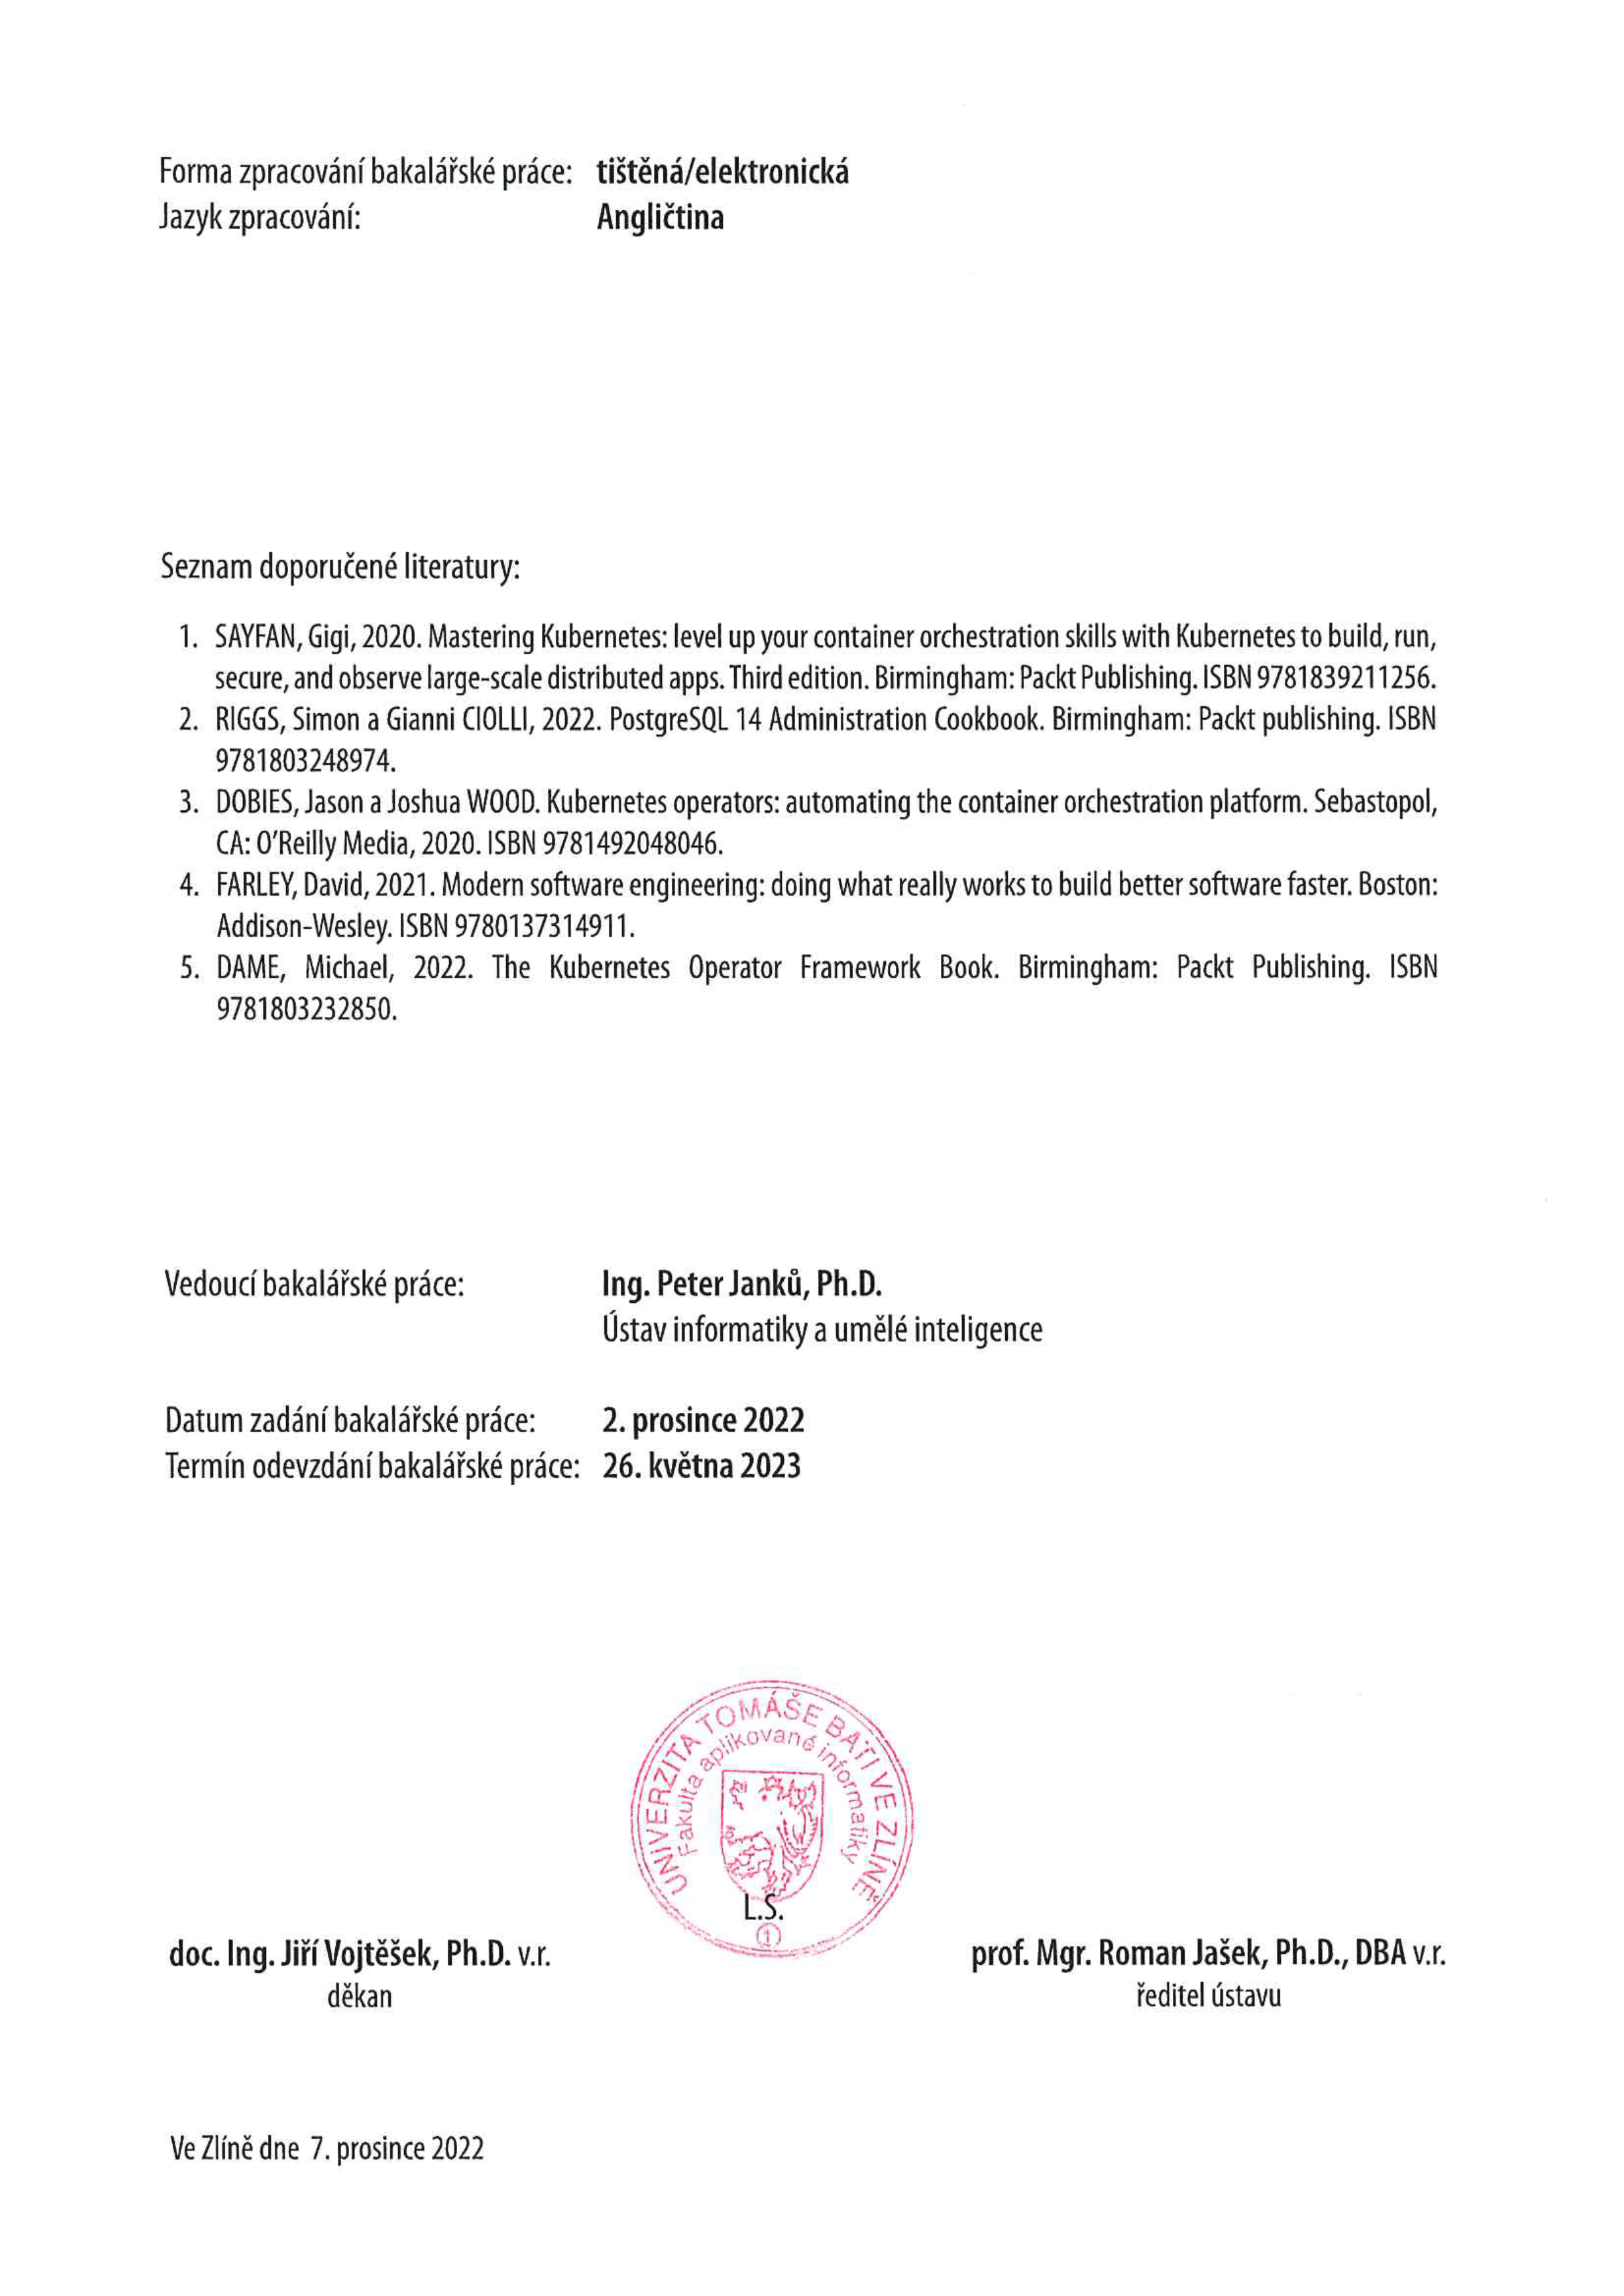
\includegraphics[width=160mm]{graphics/zadani_p2.jpg}
}

% Nastaveni zobrazovani zahlavi dokumentu
\newcommand{\aktivujZahlavi}{
	\renewcommand{\headrulewidth}{1pt}
	\rhead{\thepage}
	
	\ifczech
		\lhead{\b{UTB ve Zlíně, \ifthenelse{\equal{\fakulta}{FAI}}{Fakulta aplikované informatiky}{\ifthenelse{\equal{\fakulta}{FAME}}{Fakulta managementu a ekonomiky}{\ifthenelse{\equal{\fakulta}{FHS}}{Fakulta humanitních studií}{\ifthenelse{\equal{\fakulta}{FLKR}}{Fakulta logistiky a krizového řízení}{\ifthenelse{\equal{\fakulta}{FMK}}{Fakulta multimediálních komunikací}{\ifthenelse{\equal{\fakulta}{FT}}{Fakulta technologická}{\ifthenelse{\equal{\fakulta}{UNI}}{Univerzitní institut}{}}}}}}}}}
	\else \ifenglish
		\lhead{\b{TBU in Zlín, \ifthenelse{\equal{\fakulta}{FAI}}{Faculty of Applied Informatics}{\ifthenelse{\equal{\fakulta}{FAME}}{Faculty of Management and Economics}{\ifthenelse{\equal{\fakulta}{FHS}}{Faculty of Humanities}{\ifthenelse{\equal{\fakulta}{FLKR}}{Faculty of Logistics and Crisis Management}{\ifthenelse{\equal{\fakulta}{FMK}}{Faculty of Multimedia Communications}{\ifthenelse{\equal{\fakulta}{FT}}{Faculty of Technology}{\ifthenelse{\equal{\fakulta}{UNI}}{University Institute}{}}}}}}}}}
	\fi \fi
}

% Příkaz \logopracerok vloží na dané místo logo fakulty, typ práce a rok
\newcommand{\logopracerok}{
	\ifczech
		\iffai	\put(82.2,-223.3){\makebox(84,16.4){
\includegraphics[width=90mm]{graphics/logo/fai_logo_cz.png}}} \fi
		\iffame	\put(82.2,-223.3){\makebox(84,16.4){
\includegraphics[width=90mm]{graphics/logo/fame_logo_cz.png}}} \fi
		\iffhs	\put(82.2,-223.3){\makebox(84,16.4){
\includegraphics[width=90mm]{graphics/logo/fhs_logo_cz.png}}} \fi
		\ifflkr	\put(82.2,-223.3){\makebox(84,16.4){
\includegraphics[width=90mm]{graphics/logo/flkr_logo_cz.png}}} \fi
		\iffmk	\put(82.2,-223.3){\makebox(84,16.4){
\includegraphics[width=90mm]{graphics/logo/fmk_logo_cz.png}}} \fi
		\ifft	\put(82.2,-223.3){\makebox(84,16.4){
\includegraphics[width=90mm]{graphics/logo/ft_logo_cz.png}}} \fi
		\ifuni	\put(82.2,-223.3){\makebox(84,16.4){
\includegraphics[width=90mm]{graphics/logo/uni_logo_cz.png}}} \fi
	\else \ifenglish
		\iffai	\put(82.2,-223.3){\makebox(84,16.4){
\includegraphics[width=90mm]{graphics/logo/fai_logo_en.png}}} \fi
		\iffame	\put(82.2,-223.3){\makebox(84,16.4){
\includegraphics[width=90mm]{graphics/logo/fame_logo_en.png}}} \fi
		\iffhs	\put(82.2,-223.3){\makebox(84,16.4){
\includegraphics[width=90mm]{graphics/logo/fhs_logo_en.png}}} \fi
		\ifflkr	\put(82.2,-223.3){\makebox(84,16.4){
\includegraphics[width=90mm]{graphics/logo/flkr_logo_en.png}}} \fi
		\iffmk	\put(82.2,-223.3){\makebox(84,16.4){
\includegraphics[width=90mm]{graphics/logo/fmk_logo_en.png}}} \fi
		\ifft	\put(82.2,-223.3){\makebox(84,16.4){
\includegraphics[width=90mm]{graphics/logo/ft_logo_en.png}}} \fi
		\ifuni	\put(82.2,-223.3){\makebox(84,16.4){
\includegraphics[width=90mm]{graphics/logo/uni_logo_en.png}}} \fi
	\fi \fi
	\put(0,-205){\linethickness{1pt}\line(1,0){170}}
	\ifczech
		\ifbp \put(4,-215){\makebox(69.5,4.5)[l]{\noindent\fontsize{16}{1}\usefont{OT1}{phv}{m}{n}Bakalářská práce}} \fi
		\ifdp \put(4,-215){\makebox(69.5,4.5)[l]{\noindent\fontsize{16}{1}\usefont{OT1}{phv}{m}{n}Diplomová práce}} \fi
	\else \ifenglish
		\ifbp \put(4,-215){\makebox(69.5,4.5)[l]{\noindent\fontsize{16}{1}\usefont{OT1}{phv}{m}{n}Bachelor's thesis}} \fi
		\ifdp \put(4,-215){\makebox(69.5,4.5)[l]{\noindent\fontsize{16}{1}\usefont{OT1}{phv}{m}{n}Master's thesis}} \fi
	\fi \fi
	\put(4,-220){\makebox(69.5,4.5)[l]{\noindent\fontsize{16}{1}\usefont{OT1}{phv}{m}{n}\rok}}
	\put(0,-225){\linethickness{1pt}\line(1,0){170}}
	\put(75,-223.3){\linethickness{1pt}\line(0,1){16.4}}
}

% Úvodní stránka s logem fakulty
\newcommand{\titulnistrana}{
	\thispagestyle{empty}
	\voffset=-2.01cm\evensidemargin=0pt\oddsidemargin=0cm\parindent=0pt\headsep=0pt\headheight=0pt\parskip=0pt\textheight=272mm\textwidth=200mm
	\renewcommand{\baselinestretch}{0}
	
	\setlength{\unitlength}{1mm}
	\begin{picture}(-10,8)
		\ifczech
			% Nazev prace
			%\put(0,-100){\makebox(170,50){\fontsize{24}{1}\usefont{OT1}{phv}{b}{n}#1}}
			%		\put(0,-100){\makebox(170,50){\protect\parbox{0.8\textwidth}{\protect\centering\fontsize{24}{1}\usefont{OT1}{phv}{b}{n}#1}}}
			
			% Vyreseno odradkovani
			\put(0,-100){\makebox(170,50){\protect\parbox{0.8\textwidth}{\protect\centering\setstretch{2.0}\usefont{OT1}{phv}{b}{n}{\Huge\nazevcz}}}}
			
			% Jmeno autora
			\put(0,-135){\makebox(170,25){\fontsize{20}{1}\usefont{OT1}{phv}{m}{n}\autor}}
		\else \ifenglish
			% Nazev prace
			%\put(0,-100){\makebox(170,50){\fontsize{24}{1}\usefont{OT1}{phv}{b}{n}#1}}
			%\put(0,-95){\makebox(170,50){\protect\parbox{0.8\textwidth}{\protect\centering\fontsize{24}{1}\usefont{OT1}{phv}{b}{n}#1}}}
			%\put(0,-88)%toto bylo pouzito v pripade zobrazeni nazvu ve dvou jazycich
			\put(0,-100){\makebox(170,50){\protect\parbox{0.8\textwidth}{\protect\centering\setstretch{2.0}\usefont{OT1}{phv}{b}{n}{\Huge\nazeven}}}}
	
			%\put(0,-111){\makebox(170,50){\fontsize{20}{1}\usefont{OT1}{phv}{m}{n}#1}}
			%\put(0,-116){\makebox(170,50){\protect\parbox{0.8\textwidth}{\protect\centering\fontsize{20}{1}\usefont{OT1}{phv}{m}{n}#2}}}
			%\put(0,-115){\makebox(170,50){\protect\parbox{0.8\textwidth}{\protect\centering\setstretch{1.5}\usefont{OT1}{phv}{m}{n}{\Large\nazevcz}}}}
			
			% Jmeno autora
			\put(0,-135){\makebox(170,25){\fontsize{20}{1}\usefont{OT1}{phv}{m}{n}\autor}}
		\fi \fi
		\logopracerok
	\end{picture}
}


% Strana s abstraktem a klíčovými slovy v češtině a angličtině
\newcommand{\abstraktaklicovaslova}{
	\clearpage
	\thispagestyle{empty}
	\nm{Abstrakt}
	\abstraktcz
	
	\vspace{1cm}
	Klíčová slova: \klicovaslovacz
	
	\vspace{3cm}
	
	\nns{Abstract}
	\abstrakten
	
	\vspace{1cm}
	Keywords: \klicovaslovaen
}


% ============================================================================ %
% NASTAVENÍ ZOBRAZENÍ PŘÍLOH -- SEZNAM, ČÍSLOVÁNÍ, VLASTNÍ STYL

\makeatletter % tímto příkazem dávám najevo, že budu editovat přímo příkazy ze šablony

% definice seznamu příloh - příkaz \listofappendices
\def\listofappendices{%
	\newpage
	\phantomsection
	\setcounter{section}{0}
	\ifczech
		\addcontentsline{toc}{section}{Seznam příloh}
		\@restonecolfalse\if@twocolumn\@restonecoltrue\onecolumn\fi
		\section*{SEZNAM PŘÍLOH}
	\else \ifenglish
		\addcontentsline{toc}{section}{List of Appendices}
		\@restonecolfalse\if@twocolumn\@restonecoltrue\onecolumn\fi
		\section*{LIST OF APPENDICES}
	\fi \fi
	\@mkboth{LIST OF APPENDICES}{LIST OF APPENDICES}
	\@starttoc{loa}\if@restonecol\twocolumn\fi
	\pagestyle{empty}
	\thispagestyle{fancy}
}

\def\ext@appendix{loa}
\def\tocname{loa}

% definice příkazu \priloha{nazev prilohy} pro vložení nové přílohy
\newcommand{\priloha}[1]{
	\clearpage
	\refstepcounter{section}
	%\voffset=-3cm % vertikalni posun
	\addtocontents{loa}{\protect\makebox[1.5cm][l]{\ifczech P\else \ifenglish A\fi\fi\ \@Roman\c@section.} #1\newline}
	\ifczech
		{\bf PŘÍLOHA \ifczech P\else \ifenglish A\fi\fi\ \@Roman\c@section. \MakeTextUppercase{#1}}
	\else \ifenglish
		{\bf APPENDIX \ifczech P\else \ifenglish A\fi\fi\ \@Roman\c@section. \MakeTextUppercase{#1}}
	\fi \fi
	\par
}

% ============================================================================ %
% OBSAH: NASTAVENÍ VELKÝCH PÍSMEN PRO NÁZVY SEKCÍ A HLAVNÍCH NADPISŮ

\let\oldcontentsline\contentsline
\def\contentsline#1#2{%
	\expandafter\ifx\csname l@#1\endcsname\l@section
		\expandafter\@firstoftwo
	\else
		\expandafter\@secondoftwo
	\fi
	{%
		\oldcontentsline{#1}{\MakeTextUppercase{#2}}%
	}{%
		\oldcontentsline{#1}{#2}%
	}%
}

\def\@part[#1]#2{
	\ifnum \c@secnumdepth >\m@ne
		\refstepcounter{part}
		\addcontentsline{toc}{section}{\protect\texorpdfstring{\makebox[0.85cm]{\thepart\hfill} #1}{\thepart\ #1}}
	\else
		\addcontentsline{toc}{section}{#1}
	\fi
	{\parindent \z@ \raggedright
	\interlinepenalty \@M
	\clearpage
	\normalfont
	\ifnum \c@secnumdepth >\m@ne
		\Large\bfseries
		\nobreak
	\fi
	\vspace*{9cm}
	\center\huge \bfseries\thepart. \MakeTextUppercase{#2}
	\markboth{}{}\par}
	\nobreak
	\clearpage
	\@afterheading
}


% ============================================================================ %
% NASTAVENÍ FORMÁTU ČÍSLOVÁNÍ OBRÁZKŮ A TABULEK

\def\thefigure{\arabic{figure}}	% číslování obrázků typu (y)
\def\thetable{\arabic{table}}	% číslování tabulek typu (y)
\captiondelim{. } % změníme dvoutečku za Obr/Tab za tečku

% Nastavení číslování obrázků, tabulek i rovnic do formátu <číslo kapitoly>.<pořadové číslo>
\counterwithin{figure}{section}
\counterwithin{table}{section}
\counterwithin{equation}{section}

% Odsazeni popisku v seznamu obrazku a tabulek
\patchcmd{\@caption}{\csname the#1\endcsname}{\csname fnum@#1\endcsname}{}{}
%{\renewcommand*\numberline[1]{Fig. \,#1\space}}
%\renewcommand*\l@figure{\@dottedtocline{1}{0em}{5.0em}}
%\renewcommand*\l@table{\@dottedtocline{1}{0em}{5.0em}}

% Vynulování čítačů
\@addtoreset{table}{section}
\@addtoreset{figure}{section}
\@addtoreset{footnote}{section}

\makeatother % a to je ukončení \makeatletter


% ============================================================================ %
% ÚPRAVA VZHLEDU OBSAHU, SEZNAMU OBRÁZKŮ A TABULEK

% nastavení vertikální mezery před stylem část, nadpis 1--3
\setlength{\cftbeforepartskip}{3pt}
\setlength{\cftbeforesecskip}{3pt}
\setlength{\cftbeforesubsecskip}{3pt}
\setlength{\cftbeforesubsubsecskip}{0cm}

% odsazení zleva pro styl část, nadpis 1--3
\setlength{\cftpartindent}{0cm}
\setlength{\cftsecindent}{0cm}
\setlength{\cftsubsecindent}{0cm}
\setlength{\cftsubsubsecindent}{0cm}

% nastavení fontu pro styl část, nadpis 1--3
\renewcommand{\cftpartfont}{\small\bfseries}
\renewcommand{\cftsecfont}{\small\bfseries}
\renewcommand{\cftsubsecfont}{\scshape}
\renewcommand{\cftsubsubsecfont}{}

% odsazení čísla a textu titulku pro styl část, nadpis 1--3
\cftsetindents{part}{0cm}{1cm}
\cftsetindents{sec}{0cm}{1cm}
\cftsetindents{subsec}{0.5cm}{1.25cm}
\cftsetindents{subsubsec}{1cm}{1.5cm}
\cftsetindents{fig}{0cm}{1.5cm}
\cftsetindents{tab}{0cm}{1.5cm}

% nastavení vodící čáry pro styl část, nadpis 1--3, obrázky a tabulky
\renewcommand{\cftdot}{\ensuremath{.}} % tímto příkazem lze změnit vodící tečky v obsahu na jiný znak
\renewcommand{\cftpartleader}{\cftdotfill{0.3}}
\renewcommand{\cftsecleader}{\cftdotfill{0.3}}
\renewcommand{\cftsubsecleader}{\cftdotfill{0.3}}
\renewcommand{\cftsubsubsecleader}{\cftdotfill{0.3}}
\renewcommand{\cftfigleader}{\cftdotfill{0.3}}
\renewcommand{\cfttableader}{\cftdotfill{0.3}}

% změna fontu pro text "Obsah", "Seznam obrázků" a "Seznam tabulek"
\renewcommand{\cfttoctitlefont}{\normalsize\bfseries\thispagestyle{empty}}
\renewcommand{\cftloftitlefont}{\normalsize\bfseries\thispagestyle{fancy}}
\renewcommand{\cftlottitlefont}{\normalsize\bfseries\thispagestyle{fancy}}

\renewcommand{\cfttabpresnum}{Tab. }
\renewcommand{\cftfigaftersnum}{.}
\renewcommand{\cfttabaftersnum}{.}
\setlength{\cftfignumwidth}{5em}
\setlength{\cfttabnumwidth}{5em}


% ============================================================================ %
% NASTAVENÍ FONTU PRO NADPISY

\sectionfont{\normalsize}
\subsectionfont{\normalsize\bfseries}
\subsubsectionfont{\small\bfseries}
\paragraphfont{\small\bf}

% definice nového stylu \comment -- komentář k šabloně
\newcommand{\comment}[1]{\color{red}#1\color{black}}


% ============================================================================ %
% VSTUPY

% Nastaveni a kontrola fakulty
\newcommand{\nastavfakultu}[1]{
	\newcommand{\fakulta}{#1}
	\newif\iffai	\let\iffai\iffalse
	\newif\iffame	\let\iffame\iffalse
	\newif\iffhs	\let\iffhs\iffalse
	\newif\ifflkr	\let\ifflkr\iffalse
	\newif\iffmk	\let\iffmk\iffalse
	\newif\ifft		\let\ifft\iffalse
	\newif\ifuni	\let\ifuni\iffalse
	
	\ifthenelse{\equal{#1}{FAI}}{\let\iffai\iftrue}{}
	\ifthenelse{\equal{#1}{FAME}}{\let\iffame\iftrue}{}
	\ifthenelse{\equal{#1}{FHS}}{\let\iffhs\iftrue}{}
	\ifthenelse{\equal{#1}{FLKR}}{\let\ifflkr\iftrue}{}
	\ifthenelse{\equal{#1}{FMK}}{\let\iffmk\iftrue}{}
	\ifthenelse{\equal{#1}{FT}}{\let\ifft\iftrue}{}
	\ifthenelse{\equal{#1}{UNI}}{\let\ifuni\iftrue}{}
	
	\iffai \else \iffame \else \iffhs \else \ifflkr \else \iffmk \else \ifft \else \ifuni \else
		\errmessage{Chyba nastaveni fakulty}
	\fi \fi \fi \fi \fi \fi \fi
}

% Nastaveni a kontrola typu prace
\newcommand{\nastavtyp}[1]{
	\newcommand{\typ}{#1}
	
	\newif\ifbp \let\ifbp\iffalse
	\newif\ifdp \let\ifdp\iffalse
	
	\ifthenelse{\equal{#1}{BP}}{\let\ifbp\iftrue}{}
	\ifthenelse{\equal{#1}{DP}}{\let\ifdp\iftrue}{}
	
	\ifbp \else \ifdp \else
		\errmessage{Chyba nastaveni typu prace}
	\fi \fi
}

% Nastaveni roku
\newcommand{\nastavrok}[1]{
	\newcommand{\rok}{#1}
}

% Nastaveni jmena
\newcommand{\nastavautora}[1]{
	\newcommand{\autor}{#1}
}

% Nastaveni nazvu
\newcommand{\nastavnazevcz}[1]{
	\newcommand{\nazevcz}{#1}
}
\newcommand{\nastavnazeven}[1]{
	\newcommand{\nazeven}{#1}
}

% Nastaveni abstraktu
\newcommand{\nastavabstraktcz}[1]{
	\newcommand{\abstraktcz}{#1}
}
\newcommand{\nastavabstrakten}[1]{
	\newcommand{\abstrakten}{#1}
}

% Nastaveni klicovych slov
\newcommand{\nastavklicovaslovacz}[1]{
	\newcommand{\klicovaslovacz}{#1}
}
\newcommand{\nastavklicovaslovaen}[1]{
	\newcommand{\klicovaslovaen}{#1}
}

% Nastaveni a kontrola jazyka
\newcommand{\nastavjazyk}[1]{
	\newcommand{\jazyk}{#1}
	
	\newif\ifczech		\let\ifczech\iffalse
	\newif\ifenglish	\let\ifenglish\iffalse
	
	\ifthenelse{\equal{#1}{CZ}}{\let\ifczech\iftrue}{}
	\ifthenelse{\equal{#1}{EN}}{\let\ifenglish\iftrue}{}
	
	\ifczech \else \ifenglish \else
		\errmessage{Chyba nastaveni jazyka}
	\fi \fi
	
	\ifczech
		\usepackage[czech]{babel}
		% Vlastni definice nazvu
		\addto\captionsczech{\renewcommand{\contentsname}{\MakeTextUppercase{Obsah}}}
		\addto\captionsczech{\renewcommand{\refname}{\MakeTextUppercase{Seznam použité literatury}}}
		\addto\captionsczech{\renewcommand{\listfigurename}{\MakeTextUppercase{Seznam obrázků}}}
		\addto\captionsczech{\renewcommand{\listtablename}{\MakeTextUppercase{Seznam tabulek}}}
		%\addto\captionsczech{\renewcommand{\figurename}{Obr.}}
		%\addto\captionsczech{\renewcommand{\tablename}{Tab.}}
		\renewcommand{\cftfigpresnum}{Obr. }
	\else \ifenglish
		\usepackage[english]{babel}	
		% Vlastni definice nazvu
		\addto\captionsenglish{\renewcommand{\contentsname}{\MakeTextUppercase{Table of Contents}}}
		\addto\captionsenglish{\renewcommand{\refname}{\MakeTextUppercase{References}}}
		\addto\captionsenglish{\renewcommand{\listfigurename}{\MakeTextUppercase{List of Figures}}}
		\addto\captionsenglish{\renewcommand{\listtablename}{\MakeTextUppercase{List of Tables}}}
		%\addto\captionsenglish{\renewcommand{\figurename}{Fig.}}
		%\addto\captionsenglish{\renewcommand{\tablename}{Tab.}}
		\renewcommand{\cftfigpresnum}{Fig. }
	\fi \fi
}


% Nastaveni vertikalniho odsazeni nad rovnicemi/soustavami rovnic (prvni parametr),
% a pod (druhy parametr)
\newcommand{\nastavmezerukolemrovnic}[2]{
	\let\oldequation=\equation
	\let\endoldequation=\endequation
	\renewenvironment{equation}{\vspace{#1}\begin{oldequation}}{\end{oldequation}\vspace{#2}}
	
	\let\oldeqnarray=\eqnarray
	\let\endoldeqnarray=\endeqnarray
	\renewenvironment{eqnarray}{\vspace{#1}\begin{oldeqnarray}}{\end{oldeqnarray}\vspace{#2}}
}

% Nastaveni vertikalniho odsazeni nad tabulkami (prvni parametr),
% a pod (druhy parametr)
\newcommand{\nastavmezerukolemtabulek}[2]{
	\let\oldtable=\table
	\let\endoldtable=\endtable
	\renewenvironment{table}{\vspace{#1}\begin{oldtable}}{\end{oldtable}\vspace{#2}}
}

% Nastaveni vertikalniho odsazeni nad obrazky (prvni parametr),
% a pod (druhy parametr)
\newcommand{\nastavmezerukolemobrazku}[2]{
	\let\oldfigure=\figure
	\let\endoldfigure=\endfigure
	\renewenvironment{figure}{\vspace{#1}\begin{oldfigure}}{\end{oldfigure}\vspace{#2}}
}


% ============================================================================ %
% STRANA S PROHLASENIM

\newcommand{\prohlaseni}{{
	\clearpage
	\thispagestyle{empty}

	\ifczech
	\textbf{Prohlašuji, že}
	\begin{itemize}
		\setlength{\parskip}{0pt}
		\setlength{\itemsep}{0pt}
		\setstretch{1.05}
		\item{beru na vědomí, že odevzdáním \ifbp bakalářské \else \ifdp diplomové \fi \fi práce souhlasím se zveřejněním své práce podle zákona č. 111/1998 Sb. o vysokých školách a o změně a doplnění dalších zákonů (zákon o vysokých školách), ve znění pozdějších právních předpisů, bez ohledu na výsledek obhajoby;}
		\item{beru na vědomí, že \ifbp bakalářské \else \ifdp diplomové \fi \fi práce bude uložena v elektronické podobě v univerzitním informačním systému dostupná k prezenčnímu nahlédnutí, že jeden výtisk \ifbp bakalářské \else \ifdp diplomové \fi \fi práce bude uložen v příruční knihovně \iffai Fakulty aplikované informatiky. \else \iffame Fakulty managementu a ekonomiky. \else \iffhs Fakulty humanitních studií. \else \ifflkr Fakulty logistiky a krizového řízení. \else \iffmk Fakutly mutimediálních komunikací. \else \ifft Fakulty technologické. \else \ifuni Univerzitního institutu. \if \fi \fi \fi \fi \fi \fi \fi \fi Univerzity Tomáše Bati ve Zlíně; }
		\item{byl/a jsem seznámen/a s tím, že na moji \ifbp bakalářskou \else \ifdp diplomovou \fi \fi práci se plně vztahuje zákon č. 121/2000 Sb. o právu autorském, o právech souvisejících s právem autorským a o změně některých zákonů (autorský zákon) ve znění pozdějších právních předpisů, zejm. § 35 odst. 3;}
		\item{beru na vědomí, že podle § 60 odst. 1 autorského zákona má Univerzita Tomáše Bati ve Zlíně právo na uzavření licenční smlouvy o užití školního díla v rozsahu § 12 odst. 4 autorského zákona;}
		\item{beru na vědomí, že podle § 60 odst. 2 a 3 autorského zákona mohu užít své dílo –\ \ifbp bakalářskou \else \ifdp diplomovou \fi \fi práci nebo poskytnout licenci k~jejímu využití jen připouští-li tak licenční smlouva uzavřená mezi mnou a Univerzitou Tomáše Bati ve Zlíně s~tím, že vyrovnání případného přiměřeného příspěvku na úhradu nákladů, které byly Univerzitou Tomáše Bati ve Zlíně na vytvoření díla vynaloženy (až do jejich skutečné výše) bude rovněž předmětem této licenční smlouvy;}
		\item{beru na vědomí, že pokud bylo k vypracování \ifbp bakalářské \else \ifdp diplomové \fi \fi práce využito softwaru poskytnutého Univerzitou Tomáše Bati ve Zlíně nebo jinými subjekty pouze ke~studijním a výzkumným účelům (tedy pouze k~nekomerčnímu využití), nelze výsledky \ifbp bakalářské \else \ifdp diplomové \fi \fi práce využít ke komerčním účelům;}
		\item{beru na vědomí, že pokud je výstupem \ifbp bakalářské \else \ifdp diplomové \fi \fi práce jakýkoliv softwarový produkt, považují se za součást práce rovněž i zdrojové kódy, popř. soubory, ze kterých se projekt skládá. Neodevzdání této součásti může být důvodem k~neobhájení práce.}
	\end{itemize}
	\medskip
	%\clearpage
	%\thispagestyle{empty}
	\textbf{Prohlašuji,}
	\begin{itemize}
		\setlength{\parskip}{0pt}
		\setlength{\itemsep}{0pt}
		\setstretch{1.05}
		\item{že jsem na \ifbp bakalářské \else \ifdp diplomové \fi \fi práci pracoval samostatně a použitou literaturu jsem citoval. V případě publikace výsledků budu uveden jako spoluautor.}
		\item{že odevzdaná verze \ifbp bakalářské \else \ifdp diplomové \fi \fi práce a verze elektronická nahraná do IS/STAG jsou totožné.}
	\end{itemize}
	\medskip
	Ve Zlíně, dne \hspace{6.5cm}\dots\dots\dots\dots\dots\dots\dots\dots\dots\dots
	
	\hspace{10.3cm}podpis studenta
	
	\else \ifenglish
	%\nm{THESIS AUTHOR STATEMENT}
	\textbf{I hereby declare that:}
	\begin{itemize}
		\setlength{\parskip}{0pt}
		\setlength{\itemsep}{0pt}
		\setstretch{1.05}
		\item{I understand that by submitting my \ifbp Bachelor's \else\ifdp Master's \fi\fi thesis, I agree to the publication of my work according to Law No. 111/1998, Coll., On Universities and on changes and amendments to other acts (e.g. the Universities Act), as amended by subsequent legislation, without regard to the results of the defence of the thesis.}		
		\item{I understand that my \ifbp Bachelor's \else\ifdp Master's \fi\fi Thesis will be stored electronically in the university information system and be made available for on-site inspection, and that a copy of the \ifbp Bachelor's \else\ifdp Master's \fi\fi Thesis will be stored in the Reference Library of the 
		\iffai Faculty of Applied Informatics, \else\iffame Faculty of Management and Economics, \else \iffhs Faculty of Humanities, \else\ifflkr Faculty of Logistics and Crisis Management, \else\iffmk Faculty of Multimedia Communications, \else\ifft Faculty of Technology, \else\ifuni University Institute, \if \fi \fi \fi \fi \fi \fi \fi \fi Tomas Bata University in Zlín.}
		\item{I am aware of the fact that my \ifbp Bachelor's \else\ifdp Master's \fi\fi Thesis is fully covered by Act No. 121/2000 Coll. On Copyright, and Rights Related to Copyright, as amended by some other laws (e.g. the Copyright Act), as amended by subsequent legislation; and especially, by §35, Para. 3.}
		\item{I understand that, according to §60, Para. 1 of the Copyright Act, Tomas Bata University in Zlín has the right to conclude licensing agreements relating to the use of scholastic work within the full extent of §12, Para. 4, of the Copyright Act.}
		\item{I understand that, according to §60, Para. 2, and Para. 3, of the Copyright Act, I may use my work – \ifbp Bachelor's \else\ifdp Master's \fi\fi Thesis, or grant a license for its use, only if permitted by the licensing agreement concluded between myself and Tomas Bata University in Zlín with a view to the fact that Tomas Bata University in Zlín must be compensated for any reasonable contribution to covering such expenses/costs as invested by them in the creation of the thesis (up until the full actual amount) shall also be a subject of this licensing agreement.}
		\item{I understand that, should the elaboration of the \ifbp Bachelor's \else\ifdp Master's \fi\fi Thesis include the use of software provided by Tomas Bata University in Zlín or other such entities strictly for study and research purposes (i.e. only for non-commercial use), the results of my \ifbp Bachelor's \else\ifdp Master's \fi\fi Thesis cannot be used for commercial purposes.}
		\item{I understand that, if the output of my \ifbp Bachelor's \else\ifdp Master's \fi\fi Thesis is any software product(s), this/these shall equally be considered as part of the thesis, as well as any source codes, or files from which the project is composed. Not submitting any part of this/these component(s) may be a reason for the non-defence of my thesis.}
	\end{itemize}
	\medskip
	%\clearpage
	%\thispagestyle{empty}
	\textbf{I herewith declare that:}
	\begin{itemize}
		\setlength{\parskip}{0pt}
		\setlength{\itemsep}{0pt}
		\setstretch{1.05}
		\item{I have worked on my thesis alone and duly cited any literature I have used. In the case of the publication of the results of my thesis, I shall be listed as co-author.}
		\item{The submitted version of the thesis and its electronic version uploaded to IS/STAG are both identical.}
	\end{itemize}
	\medskip
	In Zlín; dated: \hspace{6.5cm}\dots\dots\dots\dots\dots\dots\dots\dots\dots\dots

	\hspace{10.3cm}Student's Signature
	
	\fi \fi
}}

% ============================================================================ %


% Uživatelské definice -- upravte dle požadavků
\nastavfakultu{FAI}
	% FAI  -- pro Fakultu aplikované informatiky
	% FAME -- pro Fakultu managementu a ekonomiky
	% FHS  -- pro Fakultu humanitních studií
	% FLKR -- pro Fakultu logistiky a krizového řízení
	% FMK  -- pro Fakutlu mutimediálních komunikací
	% FT   -- pro Fakultu technologickou
	% UNI  -- pro Univerzitní institut
\nastavtyp{BP}
	% BP   -- bakalářská práce
	% DP   -- diplomová práce
\nastavrok{2023}
	% zadejte rok místo "xxxx"
\nastavjazyk{EN}
	% CZ   -- práce bude v českém jazyce
	% EN   -- práce bude v anglickém jazyce

% Lze přidat vertikalni odsazeni nad (prvni parametr) a pod (druhy parametr)
% obrázky, tabulky i rovnice/soustavy rovnic
\nastavmezerukolemobrazku{0mm}{0mm} 
\nastavmezerukolemtabulek{0mm}{0mm}
\nastavmezerukolemrovnic{0mm}{0mm}

\nastavautora{Miroslav Šiřina}
\nastavnazevcz{Název práce česky (max. 2 řádky)}
\nastavnazeven{Postgres Lifecycle Management Operators in Kubernetes} % Jen u anglicky psané práce
\nastavabstraktcz{Tato bakalářská práce je zaměřena na poskytnutí doporučení zainteresovaným stranám v rámci výběru vhodného operátora pro správu životního cyklu systému Postgres v prostředí Kubernetes. Práce se zabývá životním cyklem Postgres, dále relevantními metrikami pro testování a také samotným testováním operátorů a to: Crunchy Postgres for Kubernetes, CloudNativePG, StackGres Operator a Percona Operator for PostgreSQL. Pokud jde o výkon a spolehlivost, byl Crunchy Postgres for Kubernetes doporučen jako nejvhodnější operátor. StackGres Operator byl naopak vyhodnocen jako nejlepší z hlediska jednoduchosti použití a udržovanosti. Tato práce navrhuje další studie na téma bezpečnosti operátorů životního cyklu systému Postgres v prostředí Kubernetes.}
\nastavabstrakten{This bachelor's thesis is aimed at providing recommendations to stakeholders in selecting a suitable operator for Postgres lifecycle management in a Kubernetes environment. The thesis covers the Postgres lifecycle, relevant metrics for testing, and also the testing of the operators themselves namely; Crunchy Postgres for Kubernetes, CloudNativePG, StackGres Operator, and Percona Operator for PostgreSQL. In terms of performance and reliability, Crunchy Postgres for Kubernetes was recommended as the most suitable operator. StackGres Operator, on the other hand, was rated as the best in terms of ease of use and maintenance. This thesis proposes further studies on the security of Postgres lifecycle operators in a Kubernetes environment.}
\nastavklicovaslovacz{Přehled klíčových slov}
\nastavklicovaslovaen{Some keywords}

% Následující příkaz nastaví standard PDF/A-1b
\aplikujpdfa

% ============================================================================ %
\begin{document}

\titulnistrana

\zadani

\prohlaseni

\abstraktaklicovaslova


% ============================================================================ %
\clearpage
\thispagestyle{empty}
Zde je místo pro případné poděkování, motto, úryvky knih, básní atp.


% ============================================================================ %
\obsah  % Obsah je generován automaticky


% ============================================================================ %
\OdsazovaniOdstavcuStart % Nastaví odsazování odstavců dle zvoleného jazyka

% ============================================================================ %
% Encoding: UTF-8 (žluťoučký kůň úpěl ďábelšké ódy)
% ============================================================================ %

% ============================================================================ %
\nn{Introduction}
The cloud has made our work easier. We no longer have to physically connect new machines to the network, configure network connections, add disks, or even plug in virtual ones. Kubernetes, together with the cloud, can automatically allocate new resources for our applications and, thanks to operators, can even create entire database clusters with high availability. Thanks to operators, it can also automatically set up scaling or backups. It can even restore an entire database system from a backup. This paper is focused on Kubernetes operators for the popular Postgres database management system. Its goal is to find Operators for Postgres. To evaluate their pros and cons. To test them and recommend the best one.

TBD - rewrite
% ============================================================================ %
\cast{Theory}

\n{1}{Background}
This chapter introduces the key technologies used in this thesis including Postgres, Kubernetes, and Kubernetes operators.
\n{2}{Postgres}
PostgreSQL is a powerful object-relational database management system (ORDBMS) derived from the POSTGRES package written at the University of California at Berkeley. \cite{docuPgwhatIsPg} \cite{pg14introduction} The first version of POSTGRES was released in June 1989. POSTGRES has been used in many applications, including financial data analysis systems, asteroid tracking databases, medical information database, and several geographic information systems. The size of external community users has nearly doubled by 1993. \cite{docuPgBriefHistory}

POSTGRES was using its POSTQUEL query language from version one until 1995, until Andrew Yu and Jolly Chen introduced SQL to POSTGRES. The name has changed to Postgres95. Postgres95 was completely ANSI C code reduced by 25 \% and was 30 – 50 \% faster than Postgres 4.2.  \cite{docuPgBriefHistory}

It was clear by 1996 that the name would not stand the test of time therefore it has been renamed to PostgreSQL. As stated by PostgreSQL documentation \cite{docuPgBriefHistory}: “Many people continue to refer to PostgreSQL as “Postgres” (now rarely in all capital letters) because of tradition or because it is easier to pronounce. This usage is widely accepted as a nickname or alias.“ This thesis will use Postgres as an alias for PostgreSQL as well.

More than 30 years after the first version Postgres has been considered the most used ORDBMS for professional developers by Stack Overflow survey \cite{so2022survey}. According to Riggs and Ciolli \cite{pg14introduction}: “The PostgreSQL feature set attracts serious users who have serious applications. Financial services companies may be PostgreSQL's largest user group, although governments, telecommunication companies, and many other segments are strong users as well.“ It is fully ACID compliant \cite{juba2015learningTransactionIsolation} and supports many kinds of data models such as relational, document, and key/value. \cite{pg14introduction}

\n{3}{Write Ahead Log}
Write-ahead Logging (WAL) used by Postgres is a standard technique to ensure data integrity. Its main concept is that changes in data files (where tables and indexes are stored) must only be written after they are logged (saved to a log file). That means the database is updated after the changes are written to disk. In the event of a system crash, all transactions will be recovered from the disk. \cite{docuPgWal}

Although WAL is primarily designed for recovery after a database server crash, its design also allows any changes to the database server state to be replayed backward. A copy of the log is also a form of backup. Thus, for recovery to a point in time, only logs that have been saved to that point in time can be restored. This technique is called Point-In-Time Recovery (PITR). \cite{DocuPgPITR}

\n{3}{Backup and restore}
A full set of backup commands is included in Postgres. Among the simple backup commands are pg\_dump and pg\_dumpall, which enable one or more databases to be saved in SQL format. A wide range of configuration options are available for these commands, including compression for large databases or exporting only the database schema. To restore a database from a file at a later time, the psql command can be used, which is capable of restoring a database from its dump. \cite{DocuPgDump} These commands are also helpful with migration from one major Postges version to another because the dumped files are plain SQL commands.

Because log files, mentioned earlier, contain all changes to the Database Server state, saving a copy of the log files is also a form of backup. These log files can also be streamed to other nodes to serve as a replica or backup. \cite{pg14replication}

The backup options in Postgres are quite limited. Postgres allows to set up of a backup command that runs after the next log file is created, database dumps, and log streaming. For more advanced backup techniques, additional software such as PgBackRest must be used. \cite{DocuPgPITR}

\n{4}{PgBackRest}
PgBackRest is a reliable and simple backup and restore solution that provides many features on top of classic Postgres backup and restore tools like parallel backup options with compression, local or remote backu, cloud backup (S3. Azure and Google Cloud), or backup encryption. Full, incremental, or differential backup is also supported. \cite{PGbackRest}

TBD: why is it here? Conect to crunhy and operatores


\n{3}{High Availability}
The basic structure of a database cluster consists of one or more database servers, which can be called nodes. In Postgres there are two types of nodes, primary node and standby node.  A primary node is such a node that allows reading and writing information. The newly written information is then streamed to the standby nodes. Standby nodes are read-only, they do not allow writing. \cite{pg14replication}

Achieving high availability with Postgres is possible by using more than one node in the cluster. Two options are possible here. A single primary node option, where the primary node is read and write enabled, and the other nodes are standby nodes. If the primary node is unavailable, then the standby node is promoted to the primary node. This event is called failover. In this variant, the primary node streams the logs to the standby nodes. The second option is to use multiple primary nodes. However, conflicts can occur because all primary nodes allow writes. \cite{docuPgHA}
\n{4}{Patroni}
Since Postgres does not provide any software that can detect that a node is unavailable, it is necessary to use software outside of Postgres \cite{docuPgFailover}, such as Patroni.
Patroni is a popular open-source tool created by Zalando to achieve high availability of Postgres clusters. Patroni uses a distributed configuration source such as ZooKeeper, Etcd, Consul, or Kubernetes for its operation. Patroni can automatically adjust the settings of all managed nodes, therefore it can automate failover and make it seamless. \cite{PalarkMigratingPg} \cite{PatroniDocu}


\n{3}{Load Balancing and Connection Pooling}
Using more than one node allows to direct traffic to a node that is less busy and thus achieves load balancing. Postgres doesn't come with any software that allows splitting the load on different nodes, so it is necessary to use an external load balancer such as HA Proxy or pgBouncer. The load balancer then acts as an intermediary between the database and the client and directs the traffic to the available nodes according to the set rules. These load balancers also enable connection pooling which is a technique for managing and reusing database connections to increase performance and reduce overhead. Connection pooling involves creating a pool of pre-created connections that can be shared and reused by multiple client requests, instead of creating a new connection for each request. This removes the overhead of creating a new process each time a client connects to Postgres and allows the client to use resources that would otherwise be used to service multiple requests (or complete them faster). \cite{PerconaBlogConnectionPooling}

\n{2}{Kubernetes}
Kubernetes, also known as K8s, is an open-source platform for automating deployment, scaling, and management of containerized applications. It provides a way to manage and orchestrate containers, which are units of software that package up an application and its dependencies into a single, isolated package that can run consistently on any infrastructure. \cite{vayghan2019kubernetes}

As described by Kubernetes Documentation \cite{docuKubeComponents} Kubernetes provides several key features, including:
\begin{itemize}
  \item \textbf{Service discovery:} A container can be exposed by Kubernetes either through its DNS name or its own IP address.
  \item \textbf{Load balancing:} In the case of high traffic to a container, stability of the deployment can be ensured by Kubernetes load balancing and distributing the network traffic.
  \item \textbf{Storage Orchestration:} Storage orchestration in Kubernetes allows for the automatic mounting of a storage system of choice, including local storage, public cloud providers, and others.
  \item \textbf{Automated rollouts and rollbacks:} The desired state of deployed containers can be described using Kubernetes, and the actual state can be changed to the desired state at a controlled rate. For instance, the automation of Kubernetes can be utilized to create new containers for the deployment, remove existing containers, and transfer all their resources to the newly created container.
  \item \textbf{Automatic bin packing:} A cluster of nodes for running containerized tasks is provided to Kubernetes. The amount of CPU and memory required by each container is specified to Kubernetes. The optimal utilization of resources can be achieved by Kubernetes fitting the containers onto the nodes.
  \item \textbf{Self healing:} Containers that fail are restarted by Kubernetes, those that do not respond to the user-defined health check are replaced or killed, and they are not advertised to clients until they are deemed ready to serve.
  \item \textbf{Secret and configuration management:} Sensitive information, such as passwords, OAuth tokens, and SSH keys, can be stored and managed by Kubernetes. The deployment and updating of secrets and application configuration can be done without the need to rebuild container images and without the exposure of secrets in the stack configuration.
\end{itemize}
\n{3}{Kubernetes Components}
Kubernetes cluster is composed of a set of worker machines that run containerized applications called nodes. Each cluster must have at least one node. \cite{docuKubeComponents}
\obr{The components of a Kubernetes cluster \cite{docuKubeComponents}}{}{1}{graphics/kubernetes_cluster_components.png}

The Kubernetes control plane is the management system of a Kubernetes cluster, responsible for maintaining the desired state of the cluster. It consists of multiple components that work together to manage the cluster and its resources, including pods, services, and volumes. The key components of control plane are \cite{masteringKubernetesConcepts}:
\begin{itemize}
  \item \textbf{kube-apiserver:} Acts as the front-end for the Kubernetes API and exposes the API to other components. \cite{docuKubeComponents}
  \item \textbf{etcd:} Highly available distributed key-value store that serves as the backing store for the cluster's configuration data. \cite{Dobies2020}
  \item \textbf{kube-scheduler:} Assigns work to nodes in the cluster, such as scheduling pods to run on nodes. \cite{kubeUpAndRunningPods}
  \item \textbf{kube-controller-manager:} Monitors the cluster's state and makes adjustments as necessary to maintain the desired state. \cite{masteringKubernetesConcepts}
  \item \textbf{cloud-controller-manager:} Manages cloud-related tasks such as node creation and management, volume management, and load balancing, allowing the other components of the control plane to focus on their specific responsibilities. Cloud manager is optional. Can be avoided when Kubernetes not used in cloud. \cite{docuKubeComponents}
\end{itemize}
\textbf{Node components:}
Node components in a Kubernetes cluster run on each node and provide crucial functionality for the operation of containers on that node. \cite{docuKubeComponents}
\begin{itemize}
  \item \textbf{kubelet:} Is responsible for communicating with the control plane and ensuring that containers are running and healthy. \cite{kubeUpAndRunning}
  \item \textbf{kube-proxy:} Is responsible for maintaining network rules on the nodes, allowing network communication to the containers. It enables the containers in a pod to communicate with other containers and the outside world, and performs tasks such as load balancing and traffic routing. \cite{kubeUpAndRunning}
  \item \textbf{container runtime:} Is responsible for running containers. \cite{docuKubeComponents}
\end{itemize}

\n{3}{Kubernetes Concepts}
\textcolor{cyan}{RepliceSet extension - Operators p. 28 (Replica is general and appllication agnostic) }

Pod is the smallest deployable unit that can be created in Kubernetes. \cite{docuKubePods} A Pod in Kubernetes is comprised of multiple containers and storage volumes that are run together within the same execution environment. Pods, not individual containers, are considered to be the smallest unit that can be deployed in a cluster. As a result, all containers included in a single Pod will always run on the same machine. \cite{kubeUpAndRunningPods}

A Pod's specifications are outlined in a Pod manifest, which is simply a JSON or YAML text file that represents the Kubernetes API object. Kubernetes follows a declarative configuration approach, where the system's desired state is defined in a configuration file, and the service then implements the necessary changes to make the desired state a reality. \cite{docuKubeStaticPod}

ReplicaSet’s purpose is to ensure a consistent number of replica Pods are running at all times. It is commonly used to guarantee a specified number of identical Pods are available. However, a Deployment is a more advanced concept that oversees ReplicaSets and provides a more streamlined way to make updates to Pods. It also offers additional features. As a result, it's advisable to use Deployments instead of directly utilizing ReplicaSets, unless you have specific update requirements or don't need to make updates at all. \cite{docuKubeReplicaset}

Service is an abstraction layer and defines a group of Pods and the method to access them (often referred to as a micro-service). The group of Pods targeted by a Service is usually specified through a selector. The Service abstraction makes this possible by enabling the decoupling of components. \cite{docuKubeSevice}

Kubernetes includes built-in service discovery mechanisms. When a service is created in Kubernetes, it is automatically assigned an IP address and DNS name. Clients and other services can use this name or address to access the service within the Kubernetes cluster. \cite{docuKubeSevice}

Containers and pods in Kubernetes are ephemeral. When a container is terminated, any data it has written to its own filesystem is lost. In Kubernetes, storage is represented by a basic abstraction called "volumes". Containers use these volumes by binding them to their respective pods, and can then access the storage regardless of its physical location as if it were a part of their local filesystem. \cite{masteringKubernetesStorage}

Kubernetes version 1.5 came with a new object called StatefulSet that allows a set of stateful pods to be deployed and managed. Each pod has a unique, stable network identity and a persistent storage volume. This enables stateful applications like databases to be run on Kubernetes. Advantages of using StatefulSets include predictable naming schemes, ordered pod creation and deletion, and unique persistent storage. \cite{docuKubeStatefulSet} \cite{githubKube15}

In version 1.7, Kubernetes introduced the Custom Resources extension to its API. \cite{githubIBMCr} This extension allows Kubernetes to use user-defined resources that are not native to Kubernetes as if they were native. \cite{NewStackCRDs} Custom resources (CR) is an extension to the Kubernetes API that extends the deployment with additional parameters that are not part of it. CR stores these parameters and allows the API server to access them just like the native Kubernetes parts. CR is created in the Kubernetes cluster using a definition called Custom Resource Definition (CRD). \cite{OperatorsAtK8sIface}

Kuberentes controllers are control loops\footnote[1]{A control loop is a process that continuously monitors the state of a system, compares it to a desired state, and makes adjustments to bring the system closer to the desired state.} that constantly check the state of their controlled objects. If the controlled objects are not in the desired state, the controller performs actions to get the controlled objects into that state. For example, restart a crashed node, add a new replica, modify settings, etc. \cite{docuKubeControllers}
However, to work with CR, you need to create custom controllers that can work with these resources, these controllers are called Custom Controllers. \cite{docuKubeCR}

\textcolor{red}{TBD - show that Kubernetes can run stateless very well, maybe from Operator book}


\textcolor{cyan}{TBD - Read https://containerjournal.com/kubecon-cnc-eu-2022/why-run-postgres-in-kubernetes/}

\textcolor{cyan}{TBD - Read data on Kubernetes https://dok.community/dokc-2021-report/}


\n{2}{Running Postgres in Kubernetes}
Kubernetes cannot know all complex stateful applications, which can contain a large number of nodes and have a wide range of uses while remaining general-purpose. The goal of Kubernetes is to provide an abstraction covering basic application concepts and providing options for extensions for more complex applications and their specific operations. Kubernetes cannot and should not know all the possible settings and operations that, for example, a Postgres cluster needs to run. \cite{OperatorsTeaches}

The easiest way to run Postgres in Kubernetes is through the StatefulSet just mentioned. This StatefulSet can start a Postgres pod, create a persistent volume, and connect this volume to the pod. A stateful set can do this for all replicas set in its configuration. It can also scale up or down. Unfortunately, however, all independent Postgres instances are not synchronized in any manner.

This basic setup may be sufficient for running a single node, but it is no longer sufficient for database clusters that require high availability, adjusting the settings of individual nodes, creating backups, restoring from backup, connection pooling, or even monitoring the entire cluster. For such clusters it is necessary to install other applications in the kubernetes cluster and then configure the entire Postgres cluster to work with them. This represents a large amount of work and subsequent maintenance that Kubernetes Operators can facilitate.

\n{2}{Operators}
TBD - operators capability levels

TBD - where to find operators (best operator are from the developers of postgres)

TBD - define Operator hub


As described in the previous chapters, Kubernetes can run stateless applications very well. But its general purpose makes running complex stateful applications on top of it quite challenging.


This has changed in 2016 when CoreOS came up with Operators as a way to deploy complex applications with state such as databases, caches, or monitoring systems. \cite{IArchiveCOSOperators}

An operator is a special kind of software that extends the kubernetes api and has a particular knowledge of managed software that kubernetes does not have. The Operator also serves as a packaging mechanism for distributing applications including their dependencies in Kubernetes. The Operator can manage, restore, update or monitor the software. It can also manage very complex applications. The Kubernetes Operator thus replaces the human operator after which it is named, who would otherwise take care of these tasks. \cite{OperatorsPreface} \cite{IArchiveCOSOperators}

\obr{Definition of Kubernetes Operator \cite{IArchiveCOSOperators}}{}{1}{graphics/coreos_operator.png}

CoreOS demonstrated the use of its Operator on etcd (described in the Kubernetes Components chapter). When new etcd nodes are created, it is necessary to give them a DNS names and use the etcd cluster management tools to add the new nodes to an existing cluster. CoreOS has automated these tasks with the etcd Operator so that all that is required is to increase the number of replicas in the Operator settings and the etcd Operator will perform these tasks instead of a human operator. \cite{IArchiveCOSOperators}

\n{1}{Database System Lifecycle}
The database system itself is a software like any other. It is therefore also subject to the same life cycle as software.
As depicted in figure 2.1 application lifecycle consists of three main parts. It is the governance part, development, and operations. For this thesis, only the operations part is relevant because it is the only part we are able to control.
\obr{Application Life Cycle \cite{ALM}}{}{1}{graphics/aplication-lifecycle.png}

Operation is the process of running and managing the application, which starts with deployment and continues until the application is taken out of service. This aspect of the application lifecycle management covers the release of the application into production, ongoing monitoring, and other related tasks. \cite{ALM}

TBD: connect to capability levels of Operator (define related tasks, chose the capability that would suit them all)

\n{1}{Search for Postgres Operators}
TBD: connect Operators (where to find operators)

TBD: describe CloudNativePG and Patroni

TBD: describe EDB licence

TBD: each operator security Artifact hub https://artifacthub.io/packages/olm/community-operators/postgresql

TBD: What does Percona different to Crunchy to EDB?

TBD: Postgres update every three months https://access.crunchydata.com/documentation/postgres-operator/5.3.0/tutorial/update-cluster/

TBD: Container types CloudNativePG is built on immutable application containers. What does it mean? https://cloudnative-pg.io/documentation/1.19/faq/

As previously stated in the section on Operators, the most suitable operators for a software are those developed by the software developers themselves, as they possess an in-depth understanding of the software. Regrettably, no such operator has been created for Postgres.

Operator Hub presents eight operators with varying levels of capabilities, including Crunchy Postgres for Kubernetes by Crunchy Data, EDB Postgres for Kubernetes by EnterpriseDB Corporation, Ext Postgres Operator by movetokube.com, Percona Operator for PostgreSQL by Percona, Postgres-Operator by Zalando SE, Postgresql Operator by Openlabs, and PostgreSQL Operator by Dev4Ddevs.com.

Deeper internet research revealed three more operators: CloudNativePG, StackGres, and Stolon. \cite{PostgresOnKubernetes} \cite{PalarkComparingKubernetes}

Of the eleven operators available, only five meet our minimum capability requirement of Deep Insight, namely: Crunchy Postgres for Kubernetes, EDB Postgres for Kubernetes, Percona Operator for PostgreSQL, CloudNativePG Operator, and StackGres Operator. As a result, only these five will be subjected to deeper research, testing, and evaluation.

\pagebreak
\n{2}{Crunchy Postgres for Kubernetes}
Crunchy Postgres for Kubernetes (PGO) is a Postgres Operator provided by Crunchy Data, which offers a declarative solution for the management of PostgreSQL clusters, with a focus on automation.
Crunchy Data is a company that specializes in providing open-source software solutions for Postgres. The company also provides a range of support, consulting, and training services to help organizations implement and optimize their Postgres deployment. \cite{Crunchy}:

PGO’s capabilities are the following:
\begin{itemize}
  \item \textbf{Postgres Cluster Provisioning:} PGO is able to create \cite{CrunchyDocCreate}, update \cite{CrunchyDocUpdate} or delete Postgres cluster \cite{CrunchyDocDelete}
  \item \textbf{High Availability:} High availability is achieved by adding additional nodes. PGO uses a synchronous replication technique. \cite{CrunchyDocHA}
  \item \textbf{Postgres updates:} PGO is able to apply minor patches \cite{CrunchyDocMinorUpdates}, and major upgrades since version 5.1. \cite{CrunchyBlogUpdates}
  \item \textbf{Backups:} PGO backup capabilities features: automatic backup schedules, backup to multiple locations, backup to cloud providers (AWS S3, Google Cloud Storage, Azure Blob), ad hoc backups, and backup encryption. \cite{CrunchyDocBackups}
  \item \textbf{Disaster Recovery:} PGO is capable of Point In Time recovery, in place Point in Time Recovery, restore of an individual database. \cite{CrunchyDocDisasterRecovery}
  \item \textbf{Cloning:} PGO is able to clone cluster. \cite{CrunchyDocDisasterRecovery}
  \item \textbf{Monitoring:} Monitoring is provided by Prometheus, Grafana, and Alertmanager. \cite{CrunchyDocMonitoring}
  \item \textbf{Connection Pooling:} PgBouncer connection pooler from Postgres is part of PGO. \cite{CrunchyDocConnectionPooling}
\end{itemize}

The current stable version of PGO is 5.3.0 was released on 13th January 2023 and has one critical vulnerability, 7 highly critical vulnerabilities, 31 medium, and 31 low. \cite{ArtifactHubCrunchy}
PGO is compatible with following platforms: Kubernetes 1.22-1.25, OpenShift 4.8-4.11, Rancher, Google Kubernetes Engine (GKE), including Anthos, Amazon EKS, Microsoft AKS, VMware Tanzu. \cite{CrunchyDoc}

PGO is distributed under the Apache License 2.0, an open-source license that allows for both commercial and non-commercial use. With regards to capability, PGO is considered to have the highest capability level, labeled as Autopilot. \cite{OperatorHubCrunchy}

PGO consists of the following key components \cite{CrunchyPGOGit}:
\begin{itemize}
  \item High Availability: Patroni
  \item Backups: PgBackRest
  \item Connection Pooler: PgBouncer
  \item Monitoring: PgMonitor, Prometheus, Grafana, and Alertmanager
\end{itemize}
\obr{PGO’s architecture \cite{CrunchyDocArchitecture}}{}{1}{graphics/pgo_architecture.png}


\pagebreak
\n{2}{EDB Postgres for Kubernetes}
The EDB Postgres for Kubernetes (EDBO) is a fully supported operator that has been designed, developed, and maintained by EnterpriseDB Corporation. It provides comprehensive coverage of the entire lifecycle of highly available PostgreSQL database clusters with a primary/standby architecture, utilizing native streaming replication. The operator is based on the open-source CloudNativePG operator and offers additional benefits. \cite{OperatorHubEDB}

EnterpriseDB (EDB) is a software company that provides enterprise-class PostgreSQL software and services. EDB is a leading provider of PostgreSQL technology, offering a range of products and services designed to help organizations adopt, deploy, and manage PostgreSQL databases. \cite{EDB}

As stated previously EDBO is based on open-source CloudNativePG operator. The operator that is not listed on Operator Hub. EDBO provides additional features on top of CloudNativePG operator such as support for Oracle compatibility using EDB Postgres Advanced Server, support for additional platforms such as IBM Power, and additional enterprise-grade security features. \cite{EDBdocu}

EDBO is distributed under the EDB Limited Usage License Agreement, a proprietary license that is specific to software provided by EnterpriseDB Corporation. A license key is always required for the operator to work longer than 30 days. \cite{EDBdocuLicence} Due to the restrictive nature of the license EDBO will no longer be subject to testing and evaluation but CloudNativePG will.

\pagebreak

\n{2}{CloudNativePG}
The CloudNativePG operator (CNPGO) is an operator that is available as an open-source solution and aims to manage PostgreSQL workloads across various Kubernetes clusters running in private, public, hybrid, or multi-cloud environments. The Operator aligns with DevOps principles and concepts like immutable infrastructure and declarative configuration. \cite{CNPGdocu}

Initially developed by EDB, CNPGO was later made available to the public as an open-source software under the Apache License 2.0. In April 2022, the project was submitted to CNCF Sandbox for further development and community engagement. \cite{CNPGdocu}

CNPGO’s capabilities are the following:
\begin{itemize}
  \item \textbf{Postgres Cluster Provisioning:} CNPGO is able to create, update or delete Postgres cluster. \cite{CNPGdocuCapabilityLevels}
  \item \textbf{High Availability:} High availability is achieved by adding additional nodes. PGO uses a synchronous replication technique. \cite{CNPGdocuReplication}
  \item \textbf{Direct database imports:} CNPGO provides direct database import from remote Postgres server by using pg\_dump and pg\_restore even on different Postgres versions. \cite{CNPGdocuDatabaseImports}
  \item \textbf{Postgres updates:} CNPGO is able to apply minor patches. \cite{CNPGdocuUpdates} Major updates are possible by previously mentioned Direct database imports.
  \item \textbf{Backups:} CNPGO backup capabilities features: automatic backup schedules, backup to multiple locations, backup to cloud providers (AWS S3, Google Cloud Storage, Azure Blob), on-demand backups, and backup encryption \cite{CNPGdocuBackup}\cite{CNPGdocuTDE}. Due to EDB’s backup software Barman backup compression is available also. \cite{CNPGdocuBackup}
  \item \textbf{Disaster Recovery:} CNPGO is capable of Point In Time recovery. Database recovery was not mentioned in the documentation. \cite{CNPGdocuBackup}
  \item \textbf{Cloning:} CNPGO is able to create cluster replicas. \cite{CNPGdocuReplication}
  \item \textbf{Monitoring:} Monitoring can be provided by the additional installation of Prometheus, and Grafana, and Alertmanager. \cite{CNPGdocuQuickstart}
  \item \textbf{Connection Pooling:} Is provided by native Postgres pooler PgBouncer. \cite{CNPGdocuConnectionPooling}
  \item \textbf{Customization:} CNPGO provides a wide area of Postgres customization such as max parallel workers tuning or WAL configuration \cite{CNPGdocuConfiguration}
\end{itemize}

The current major stable version of CNPGO is 1.19 was released on 14th February 2023. CNPGO is distributed under the Apache License 2.0 open-source license. CNPGO is considered to have the highest capability level, labeled as Autopilot. \cite{CNPGdocu}

CNPGO consists of the following key components \cite{PostgresOnKubernetes} \cite{CNPGdocuQuickstart}:
\begin{itemize}
  \item High Availability: Postgres instance manager
  \item Backups: Barman
  \item Connection Pooler: PgBouncer
  \item Monitoring: Prometheus, Grafana, and Alertmanager
\end{itemize}

\obr{CNPGO’s architecture \cite{CNPGdocuConnectionPooling}}{}{1}{graphics/CNPGO_architecture.png}

\pagebreak
\n{2}{StackGres Operator}
StackGres (SPGO) is a comprehensive distribution of PostgreSQL for Kubernetes, delivered in a user-friendly deployment package. The distribution includes a set of PostgreSQL components that have been carefully selected and optimized to work seamlessly with each other. \cite{SPGOgitlab}

SPGO is developed by OnGres that was established as a result of years of experience in working with and creating products based on Postgres and supporting clients with their Postgres infrastructures. Postgres databases are at the heart of the company's business, as the name suggests. \cite{OnGres}

SPGO’s capabilities are the following \cite{OnGres}:
\begin{itemize}
  \item \textbf{Postgres Cluster Provisioning:} SPGO is able to create, update or delete Postgres cluster.
  \item \textbf{High Availability:} High availability is achieved by adding additional nodes.
  \item \textbf{Postgres updates:} SPGO is able to apply minor patches. Major updates are possible by SGDbOps \cite{SPGODocuMajorUpdates}.
  \item \textbf{Backups:} SPGO backup capabilities features: automatic backup schedules, backup to multiple locations, backup to cloud providers (AWS S3, Google Cloud Storage, Azure Blob)
  \item \textbf{Disaster Recovery:} SPGO is capable of Point In Time recovery. Database recovery was not mentioned in the documentation.
  \item \textbf{Cloning:} SPGO is able to create cluster replicas.
  \item \textbf{Monitoring:} Monitoring is provided by Prometheus, Grafana, and Alertmanager.
  \item \textbf{Connection Pooling:} Is provided by native Postgres pooler PgBouncer.
  \item \textbf{Customization:} SPGO provides a wide area of Postgres customization such as WAL configuration, archive mode, vacuum, etc. \cite{SPGODocuCustomization}
  \item \textbf{Mamagement Console:} SPGO provides a fully featured management web console.

\end{itemize}

The current stable version of SPGO is 1.4.2 was released on 24th January 2022. \cite{ SPGOgitlabChangelog} SPGO is distributed under the AGPL3 open-source license. \cite{SPGODocuLicence} SPGO capability level hasn’t been mentioned in the documentation or its web pages.

SPGO consists of the following key components \cite{PostgresOnKubernetes}:
\begin{itemize}
  \item High Availability: Patroni
  \item Backups: WAL-G
  \item Connection Pooler: PgBouncer
  \item Monitoring: Prometheus, Grafana, and Alertmanager.
\end{itemize}


\obr{SPGO’s architecture \cite{SPGOdocuArchitecture}}{}{1}{graphics/SPGO_architecture.png}

\pagebreak
\n{2}{Percona Operator for PostgreSQL}
Percona is a company that provides services and solutions for open-source database technologies. It offers expertise, support, and software for MySQL, MongoDB, and PostgreSQL. The company's offerings help organizations manage their open-source databases and ensure optimal performance, security, and scalability. \cite{Percona}

Percona Operator for PostgreSQL (PPO) is based on Crunchy Postgres for Kubernetes. Percona forked PGO v 4.7 and has added enhancements for monitoring, upgradability, and flexibility. \cite{PerconaBlogProsAndCons}

Differences between PGO and PPO are the following:
\begin{itemize}
  \item \textbf{Postgres updates:} PPO provides automatic Postgres updates for minor and major versions of Postgres.  \cite{PerconaDocuUpdate}
  \item \textbf{Backups:} PPO is not able to back up to Azure. \cite{PerconaDocuCompare}
  \item \textbf{Disaster Recovery:} PPO documentation does not mention the possibility of restoring a single database from a backup. \cite{PerconaDocuBackups}
  \item \textbf{Monitoring:} PPO is not using the usual monitoring stack consisting of Prometheus and Grafana but their own Percona Monitoring and Management. \cite{PerconaDocuMonitoring}
\end{itemize}

The current stable version of PPO is 1.3.0 was released on 4th August 2022. The upcoming version 2.0.0 is not yet production ready therefore will not be subject to testing and evaluation. \cite{PerconaDocuV2} PPO is distributed under the Apache License 2.0, an open-source license that allows for both commercial and non-commercial use. With regards to capability, PPO is considered to have the second highest capability level, labeled as Deep Insights. \cite{OperatorHubPercona}

PPO consists of the following key components \cite{PostgresOnKubernetes}:
\begin{itemize}
  \item High Availability: Patroni
  \item Backups: PgBackRest
  \item Connection Pooler: PgBouncer
  \item Monitoring: Percona Monitoring and Management
\end{itemize}
\obr{PPO’s architecture \cite{CrunchyDocArchitecture}}{}{1}{graphics/PPO_architecture.png}




\tab{Comparison of selected Operators}{tab:priklad2}{1}{|l|l|l|l|l|}{
  \hline
  & PGO 5.3.0 & CNPGO 1.18.1 & SPGO 1.4.2 & PPO 1.3.0\\ \hline
  Programing language & GO & GO & JAVA & GO\\ \hline
  Supported Postgres versions & 12, 13, 14, 15 & 11, 12, 13, 14, 15 & 12, 13, 14, 15 & 12, 13, 14\\ \hline
  Major version update & Manual & Manual & Manual & Automatic\\ \hline
  Licence & Apache 2.0 & Apache 2.0 & Apache 2.0 & AGPL 3\\ \hline
  User interface &  No & No & Yes & No\\ \hline
}

% \emph{F} & (jedna) & (dva) & (tři) & (čtyři) & (pět) & 300 \\ \hline



\n{1}{Architecture}
%\obr{2022 Developer Survey \cite{so2022survey}}{}{1}{graphics/postgres_stack_overflow_survey.png}





\n{1}{Nadpisy a podnadpisy}
Na této stránce je k vidění způsob tvorby různých úrovní nadpisů.

\n{2}{Podnadpis A}
Text

\n{2}{Podnadpis B}
Text

\n{2}{Podnadpis C}
Text

\n{3}{Podpodnadpis alfa}
Text

\n{3}{Podpodnadpis beta}
Text

\n{3}{Podpodnadpis gama}
Text

\n{2}{Podnadpis D}
Text


\n{1}{Vkládání obrázků, tabulek a citací}
Níže následují ukázky vložení obrázku, tabulky a různorodých citací.


\n{2}{Obrázek}
Obrázek \ref{fig:logo} prezentuje logo Fakulty aplikované informatiky.

% Obrázek lze vkládat pomocí následujícího zjednodušeného stylu, nebo klasickým LaTex způsobem
% Pozor! Obrázek nesmí obsahovat alfa kanál (průhlednost). Jde to totiž proti požadovanému standardu PDF/A.
\obr{Popisek obrázku}{fig:logo}{0.5}{graphics/logo/fai_logo_cz.png}


\n{2}{Tabulka}
Tabulka \ref{tab:priklad} obsahuje dva řádky a celkem 7 sloupců.

% Tabulku lze vkládat pomocí následujícího zjednodušeného stylu, nebo klasickým LaTex způsobem
\tab{Popisek tabulky}{tab:priklad}{0.65}{|l|c|c|c|c|c|r|}{
  \hline
  & 1 & 2 & 3 & 4 & 5 & Cena [Kč] \\ \hline
  \emph{F} & (jedna) & (dva) & (tři) & (čtyři) & (pět) & 300 \\ \hline
}

% ============================================================================ %

% Pokud Vaše práce obsahuje analytickou část, stačí odkomentovat nasledujících dva řádky
%\cast{Analytická část}
%\n{1}{Nadpis}


% ============================================================================ %
\cast{Praktická část}
\n{1}{Nadpis první kapitoly praktické části}
Text je text


% ============================================================================ %
\nn{Závěr}
Text závěru.


% ============================================================================ %
 % Hlavni text prace

\OdsazovaniOdstavcuStop


% ============================================================================ %
\seznamlitbib


% ============================================================================ %
% ============================================================================ %
% Encoding: UTF-8 (žluťoučký kůň úpěl ďábelšké ódy)
% ============================================================================ %

\seznamzkr

\begin{tabular}{ll}
  ACID   & Atomicity, Consistency, Isolation, Durability \\
  API    & Application Programming Interface             \\
  CNPGO  & CloudNativePG                                 \\
  CR     & Custom Resource                               \\
  CRD    & Custom Resource Definition                    \\
  EDBO   & EDB Postgres for Kubernetes Operator          \\
  K8s    & Kubernetes                                    \\
  ORDBMS & Object-relational Database Management System  \\
  PGO    & Crunchy Postgres for Kubernetes               \\
  PPO    & Percona Operator for PostgreSQL               \\
  RBAC   & Role-Based Acceess Control                    \\
  SPGO   & StackGres Operator                            \\
  WAL    & Write Ahead Log                               \\
\end{tabular}

% ============================================================================ %
 % Seznam zkratek


% ============================================================================ %
\seznamobr  % Seznam je generován automaticky


% ============================================================================ %
\seznamtab  % Seznam je generován automaticky


% ============================================================================ %
% ============================================================================ %
% Encoding: UTF-8 (žluťoučký kůň úpěl ďábelšké ódy)
% ============================================================================ %

\listofappendices

\priloha{Název přílohy}
Obsah přílohy


% ============================================================================ %
 % Prilohy


% ============================================================================ %

\end{document}

% ============================================================================ %
